% Options for packages loaded elsewhere
\PassOptionsToPackage{unicode}{hyperref}
\PassOptionsToPackage{hyphens}{url}
\documentclass[
]{book}
\usepackage{xcolor}
\usepackage{amsmath,amssymb}
\setcounter{secnumdepth}{-\maxdimen} % remove section numbering
\usepackage{iftex}
\ifPDFTeX
  \usepackage[T1]{fontenc}
  \usepackage[utf8]{inputenc}
  \usepackage{textcomp} % provide euro and other symbols
\else % if luatex or xetex
  \usepackage{unicode-math} % this also loads fontspec
  \defaultfontfeatures{Scale=MatchLowercase}
  \defaultfontfeatures[\rmfamily]{Ligatures=TeX,Scale=1}
\fi
\usepackage{lmodern}
\ifPDFTeX\else
  % xetex/luatex font selection
\fi
% Use upquote if available, for straight quotes in verbatim environments
\IfFileExists{upquote.sty}{\usepackage{upquote}}{}
\IfFileExists{microtype.sty}{% use microtype if available
  \usepackage[]{microtype}
  \UseMicrotypeSet[protrusion]{basicmath} % disable protrusion for tt fonts
}{}
\makeatletter
\@ifundefined{KOMAClassName}{% if non-KOMA class
  \IfFileExists{parskip.sty}{%
    \usepackage{parskip}
  }{% else
    \setlength{\parindent}{0pt}
    \setlength{\parskip}{6pt plus 2pt minus 1pt}}
}{% if KOMA class
  \KOMAoptions{parskip=half}}
\makeatother
\usepackage{graphicx}
\makeatletter
\newsavebox\pandoc@box
\newcommand*\pandocbounded[1]{% scales image to fit in text height/width
  \sbox\pandoc@box{#1}%
  \Gscale@div\@tempa{\textheight}{\dimexpr\ht\pandoc@box+\dp\pandoc@box\relax}%
  \Gscale@div\@tempb{\linewidth}{\wd\pandoc@box}%
  \ifdim\@tempb\p@<\@tempa\p@\let\@tempa\@tempb\fi% select the smaller of both
  \ifdim\@tempa\p@<\p@\scalebox{\@tempa}{\usebox\pandoc@box}%
  \else\usebox{\pandoc@box}%
  \fi%
}
% Set default figure placement to htbp
\def\fps@figure{htbp}
\makeatother
\setlength{\emergencystretch}{3em} % prevent overfull lines
\providecommand{\tightlist}{%
  \setlength{\itemsep}{0pt}\setlength{\parskip}{0pt}}
\usepackage{bookmark}
\IfFileExists{xurl.sty}{\usepackage{xurl}}{} % add URL line breaks if available
\urlstyle{same}
\hypersetup{
  hidelinks,
  pdfcreator={LaTeX via pandoc}}

\author{}
\date{}

\begin{document}
\frontmatter

\mainmatter
\chapter{Visualisasi dan Perhitungan Geometri dengan EMT}\label{visualisasi-dan-perhitungan-geometri-dengan-emt}

Euler menyediakan beberapa fungsi untuk melakukan visualisasi dan perhitungan geometri, baik secara numerik maupun analitik (seperti biasanya tentunya, menggunakan Maxima). Fungsi-fungsi untuk visualisasi dan perhitungan geometeri tersebut disimpan di dalam file program ``geometry.e'', sehingga file tersebut harus dipanggil sebelum menggunakan fungsi-fungsi atau perintah-perintah untuk geometri.

\textgreater load geometry

\begin{verbatim}
Numerical and symbolic geometry.
\end{verbatim}

\section{Fungsi-fungsi Geometri}\label{fungsi-fungsi-geometri}

Fungsi-fungsi untuk Menggambar Objek Geometri:

defaultd:=textheight()*1.5: nilai asli untuk parameter d\\
setPlotrange(x1,x2,y1,y2): menentukan rentang x dan y pada bidang

koordinat

setPlotRange(r): pusat bidang koordinat (0,0) dan batas-batas sumbu-x dan y adalah -r sd r

plotPoint (P, ``P''): menggambar titik P dan diberi label ``P''

plotSegment (A,B, ``AB'', d): menggambar ruas garis AB, diberi label ``AB'' sejauh d

plotLine (g, ``g'', d): menggambar garis g diberi label ``g'' sejauh d

plotCircle (c,``c'',v,d): Menggambar lingkaran c dan diberi label ``c''

plotLabel (label, P, V, d): menuliskan label pada posisi P

Fungsi-fungsi Geometri Analitik (numerik maupun simbolik):

turn(v, phi): memutar vektor v sejauh phi\\
turnLeft(v): memutar vektor v ke kiri\\
turnRight(v): memutar vektor v ke kanan\\
normalize(v): normal vektor v\\
crossProduct(v, w): hasil kali silang vektorv dan w.\\
lineThrough(A, B): garis melalui A dan B, hasilnya {[}a,b,c{]} sdh.

ax+by=c.

lineWithDirection(A,v): garis melalui A searah vektor v

getLineDirection(g): vektor arah (gradien) garis g

getNormal(g): vektor normal (tegak lurus) garis g

getPointOnLine(g): titik pada garis g

perpendicular(A, g): garis melalui A tegak lurus garis g

parallel (A, g): garis melalui A sejajar garis g

lineIntersection(g, h): titik potong garis g dan h

projectToLine(A, g): proyeksi titik A pada garis g

distance(A, B): jarak titik A dan B

distanceSquared(A, B): kuadrat jarak A dan B

quadrance(A, B): kuadrat jarak A dan B

areaTriangle(A, B, C): luas segitiga ABC

computeAngle(A, B, C): besar sudut \textless ABC

angleBisector(A, B, C): garis bagi sudut \textless ABC

circleWithCenter (A, r): lingkaran dengan pusat A dan jari-jari r

getCircleCenter(c): pusat lingkaran c

getCircleRadius(c): jari-jari lingkaran c

circleThrough(A,B,C): lingkaran melalui A, B, C

middlePerpendicular(A, B): titik tengah AB

lineCircleIntersections(g, c): titik potong garis g dan lingkran c

circleCircleIntersections (c1, c2): titik potong lingkaran c1 dan c2

planeThrough(A, B, C): bidang melalui titik A, B, C

Fungsi-fungsi Khusus Untuk Geometri Simbolik:

getLineEquation (g,x,y): persamaan garis g dinyatakan dalam x dan y\\
getHesseForm (g,x,y,A): bentuk Hesse garis g dinyatakan dalam x dan

y dengan titik A pada

sisi positif (kanan/atas) garis

quad(A,B): kuadrat jarak AB

spread(a,b,c): Spread segitiga dengan panjang sisi-sisi a,b,c, yakni sin(alpha)\^{}2 dengan

alpha sudut yang menghadap sisi a.

crosslaw(a,b,c,sa): persamaan 3 quads dan 1 spread pada segitiga dengan panjang sisi a, b, c.

triplespread(sa,sb,sc): persamaan 3 spread sa,sb,sc yang memebntuk suatu segitiga

doublespread(sa): Spread sudut rangkap Spread 2*phi, dengan sa=sin(phi)\^{}2 spread a.

\section{Contoh 1: Luas, Lingkaran Luar, Lingkaran Dalam Segitiga}\label{contoh-1-luas-lingkaran-luar-lingkaran-dalam-segitiga}

Untuk menggambar objek-objek geometri, langkah pertama adalah menentukan rentang sumbu-sumbu koordinat. Semua objek geometri akan digambar pada satu bidang koordinat, sampai didefinisikan bidang koordinat yang baru.

\textgreater setPlotRange(-0.5,2.5,-0.5,2.5): // mendefinisikan bidang koordinat baru

\begin{figure}
\centering
\pandocbounded{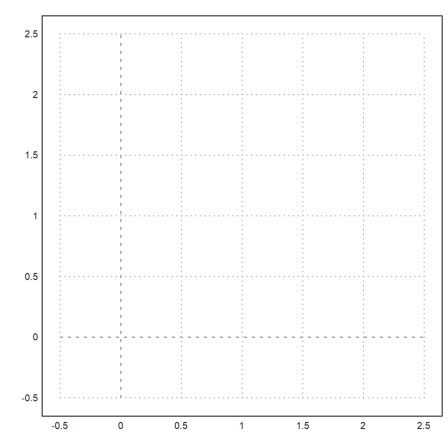
\includegraphics[keepaspectratio]{images/EMT4Geometry - Naila Khalidatus Salwa-001.png}}
\caption{images/EMT4Geometry\%20-\%20Naila\%20Khalidatus\%20Salwa-001.png}
\end{figure}

\section{Menggambar titik dan ruas garis}\label{menggambar-titik-dan-ruas-garis}

Sekarang tetapkan tiga titik dan gambarkan plotnya.

\textgreater A={[}1,0{]}; plotPoint(A,``A''): // definisi dan gambar tiga titik

\begin{figure}
\centering
\pandocbounded{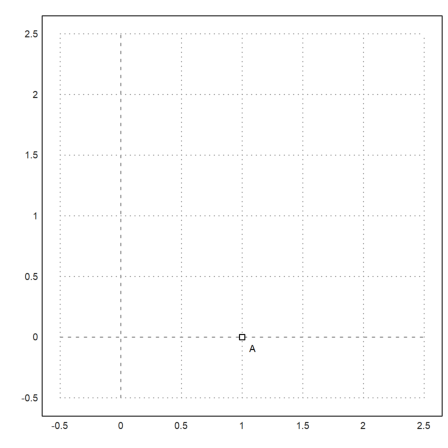
\includegraphics[keepaspectratio]{images/EMT4Geometry - Naila Khalidatus Salwa-002.png}}
\caption{images/EMT4Geometry\%20-\%20Naila\%20Khalidatus\%20Salwa-002.png}
\end{figure}

\textgreater B={[}0,1{]}; plotPoint(B,``B''):

\begin{figure}
\centering
\pandocbounded{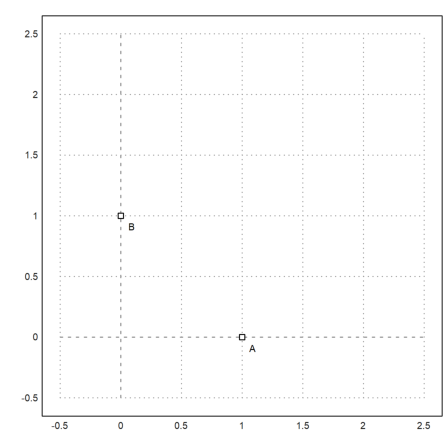
\includegraphics[keepaspectratio]{images/EMT4Geometry - Naila Khalidatus Salwa-003.png}}
\caption{images/EMT4Geometry\%20-\%20Naila\%20Khalidatus\%20Salwa-003.png}
\end{figure}

\textgreater C={[}2,2{]}; plotPoint(C,``C''):

\begin{figure}
\centering
\pandocbounded{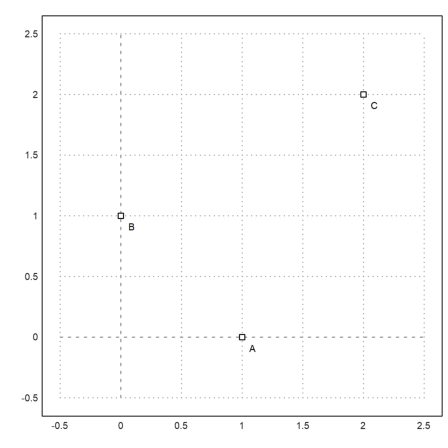
\includegraphics[keepaspectratio]{images/EMT4Geometry - Naila Khalidatus Salwa-004.png}}
\caption{images/EMT4Geometry\%20-\%20Naila\%20Khalidatus\%20Salwa-004.png}
\end{figure}

Lalu tiga segmen.

\textgreater plotSegment(A,B,``c'');

\textgreater plotSegment(B,C,``a''); // a=BC

\textgreater plotSegment(A,C,``b''): // b=AC

\begin{figure}
\centering
\pandocbounded{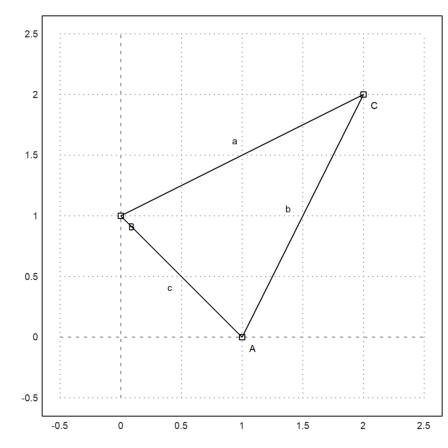
\includegraphics[keepaspectratio]{images/EMT4Geometry - Naila Khalidatus Salwa-005.png}}
\caption{images/EMT4Geometry\%20-\%20Naila\%20Khalidatus\%20Salwa-005.png}
\end{figure}

Fungsi geometri meliputi fungsi untuk membuat garis dan lingkaran. Format garisnya adalah {[}a,b,c{]} yang mewakili garis dengan persamaan ax+by=c.

\section{Menggambar garis yang melalui 2 titik}\label{menggambar-garis-yang-melalui-2-titik}

\textgreater lineThrough(B,C) // garis yang melalui B dan C

\begin{verbatim}
[-1,  2,  2]
\end{verbatim}

Hitung garis tegak lurus yang melalui A di BC.

\textgreater h=perpendicular(A,lineThrough(B,C)); // garis h tegak lurus BC melalui A

Dan persimpangannya dengan BC.

\section{Menggambar titik potong}\label{menggambar-titik-potong}

\textgreater D=lineIntersection(h,lineThrough(B,C)); // D adalah titik potong h dan BC

Buat plotnya.

\textgreater plotPoint(D,value=1); // koordinat D ditampilkan

\textgreater aspect(1); plotSegment(A,D): // tampilkan semua gambar hasil plot\ldots()

\begin{figure}
\centering
\pandocbounded{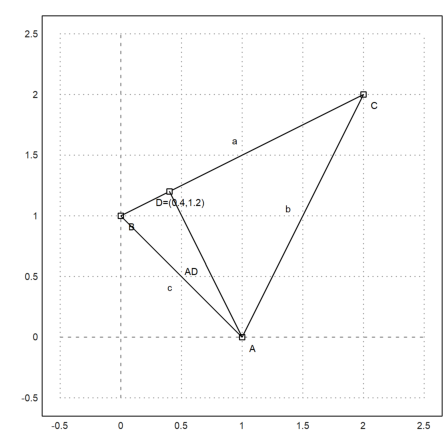
\includegraphics[keepaspectratio]{images/EMT4Geometry - Naila Khalidatus Salwa-006.png}}
\caption{images/EMT4Geometry\%20-\%20Naila\%20Khalidatus\%20Salwa-006.png}
\end{figure}

\section{Menghitung luas segitiga ABC}\label{menghitung-luas-segitiga-abc}

\[L_{\triangle ABC}= \frac{1}{2}AD.BC.\]\textgreater norm(A-D)*norm(B-C)/2 // AD=norm(A-D), BC=norm(B-C)

\begin{verbatim}
1.5
\end{verbatim}

Bandingkan dengan rumus determinan dari 3 titik yang sudah diketahui, yaitu A(1,0), B(0,1), C(2,2), dengan rumus:

\[\frac{1}{2} [x_1(y_2-y_3)+x_2(y_3-y_1)+x_3(y_1-y_2)\]\textgreater areaTriangle(A,B,C) // hitung luas segitiga langusng dengan fungsi

\begin{verbatim}
1.5
\end{verbatim}

Cara lain menghitung luas segitigas ABC:

\textgreater distance(A,D)*distance(B,C)/2

\begin{verbatim}
1.5
\end{verbatim}

\section{Menentukan besar sudut}\label{menentukan-besar-sudut}

Sudut di C.

\textgreater degprint(computeAngle(B,C,A))

\begin{verbatim}
36°52'11.63''
\end{verbatim}

\section{Menggambar lingkaran luar segitiga}\label{menggambar-lingkaran-luar-segitiga}

\textgreater c=circleThrough(A,B,C); // lingkaran luar segitiga ABC

\textgreater R=getCircleRadius(c); // jari2 lingkaran luar

\textgreater O=getCircleCenter(c); // titik pusat lingkaran c

\textgreater plotPoint(O,``O''); // gambar titik ``O''

\textgreater plotCircle(c,``Lingkaran luar segitiga ABC''):

\begin{figure}
\centering
\pandocbounded{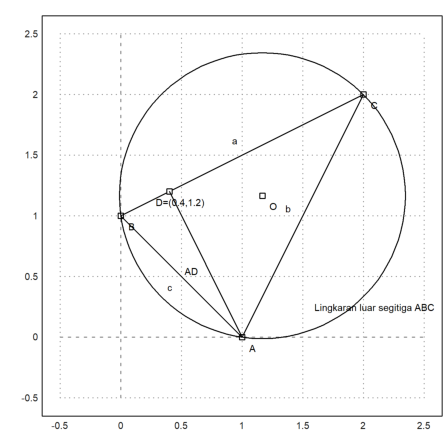
\includegraphics[keepaspectratio]{images/EMT4Geometry - Naila Khalidatus Salwa-009.png}}
\caption{images/EMT4Geometry\%20-\%20Naila\%20Khalidatus\%20Salwa-009.png}
\end{figure}

Tampilkan koordinat titik pusat dan jari-jari lingkaran luar.

\textgreater O, R

\begin{verbatim}
[1.16667,  1.16667]
1.17851130198
\end{verbatim}

\section{Menggambar lingkaran dalam segitiga}\label{menggambar-lingkaran-dalam-segitiga}

Sekarang akan digambar lingkaran dalam segitiga ABC. Titik pusat lingkaran dalam adalah titik potong garis-garis bagi sudut.

\textgreater l=angleBisector(A,C,B); // garis bagi \textless ACB

\textgreater g=angleBisector(C,A,B); // garis bagi \textless CAB

\textgreater P=lineIntersection(l,g) // titik potong kedua garis bagi sudut

\begin{verbatim}
[0.86038,  0.86038]
\end{verbatim}

Tambahkan semuanya ke plot.

\textgreater color(5); plotLine(l); plotLine(g); color(1); // gambar kedua garis bagi sudut

\textgreater plotPoint(P,``P''); // gambar titik potongnya

\textgreater r=norm(P-projectToLine(P,lineThrough(A,B))) // jari-jari lingkaran dalam

\begin{verbatim}
0.509653732104
\end{verbatim}

\textgreater S= circleWithCenter(P,r), ``Lingkaran dalam segitiga ABC'';

\begin{verbatim}
[0.86038,  0.86038,  0.509654]
\end{verbatim}

\textgreater plotCircle(S): // gambar lingkaran dalam

\begin{figure}
\centering
\pandocbounded{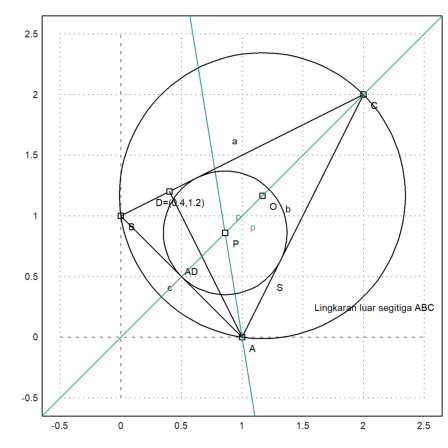
\includegraphics[keepaspectratio]{images/EMT4Geometry - Naila Khalidatus Salwa-010.png}}
\caption{images/EMT4Geometry\%20-\%20Naila\%20Khalidatus\%20Salwa-010.png}
\end{figure}

\section{Latihan}\label{latihan}

\begin{enumerate}
\def\labelenumi{\arabic{enumi}.}
\tightlist
\item
  Tentukan ketiga titik singgung lingkaran dalam dengan sisi-sisi segitiga ABC.
\end{enumerate}

\textgreater setPlotRange(-2.5,4.5,-2.5,4.5);

\textgreater A={[}-2,1{]}; plotPoint(A,``A'');

\textgreater B={[}1,-2{]}; plotPoint(B,``B'');

\textgreater C={[}4,4{]}; plotPoint(C,``C'');

\begin{enumerate}
\def\labelenumi{\arabic{enumi}.}
\setcounter{enumi}{1}
\tightlist
\item
  Gambar segitiga dengan titik-titik sudut ketiga titik singgung tersebut. Merupakan segitiga apakah itu?
\end{enumerate}

\textgreater plotSegment(A,B,``c'')

\textgreater plotSegment(B,C,``a'')

\textgreater plotSegment(A,C,``b'')

\textgreater aspect(1):

\begin{figure}
\centering
\pandocbounded{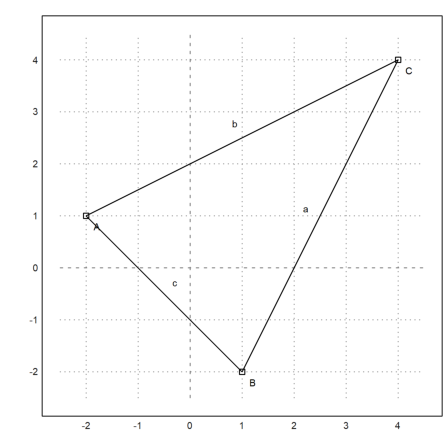
\includegraphics[keepaspectratio]{images/EMT4Geometry - Naila Khalidatus Salwa-011.png}}
\caption{images/EMT4Geometry\%20-\%20Naila\%20Khalidatus\%20Salwa-011.png}
\end{figure}

Dapat dilihat bahwa segitiga tersebut adalah segitiga sama kaki.

\begin{enumerate}
\def\labelenumi{\arabic{enumi}.}
\setcounter{enumi}{2}
\tightlist
\item
  Hitung luas segitiga tersebut.
\end{enumerate}

\textgreater areaTriangle(A,B,C)

\begin{verbatim}
13.5
\end{verbatim}

\begin{enumerate}
\def\labelenumi{\arabic{enumi}.}
\setcounter{enumi}{3}
\tightlist
\item
  Tunjukkan bahwa garis bagi sudut yang ke tiga juga melalui titik pusat lingkaran dalam.
\end{enumerate}

\textgreater l=angleBisector(A,C,B);

\textgreater g=angleBisector(C,A,B);

\textgreater P=lineIntersection(l,g)

\begin{verbatim}
[0.581139,  0.581139]
\end{verbatim}

\textgreater color(3); plotLine(l); plotLine(g); color(1);

\textgreater plotPoint(P,``P'');

\textgreater r=norm(P-projectToLine(P,lineThrough(A,B)))

\begin{verbatim}
1.52896119631
\end{verbatim}

\textgreater plotCircle(circleWithCenter(P,r),``Lingkaran dalam segitiga ABC''):

\begin{figure}
\centering
\pandocbounded{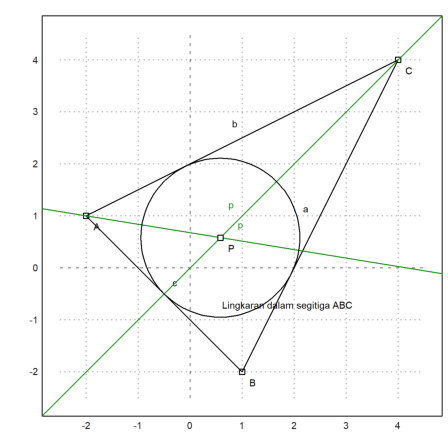
\includegraphics[keepaspectratio]{images/EMT4Geometry - Naila Khalidatus Salwa-012.png}}
\caption{images/EMT4Geometry\%20-\%20Naila\%20Khalidatus\%20Salwa-012.png}
\end{figure}

Terbukti bahwa garis bagi sudut yang ketiga juga melalui titik pusat lingkaran dalam.

\begin{enumerate}
\def\labelenumi{\arabic{enumi}.}
\setcounter{enumi}{4}
\tightlist
\item
  Gambar jari-jari lingkaran dalam.
\end{enumerate}

\textgreater r=norm(P-projectToLine(P,lineThrough(A,B)))

\begin{verbatim}
1.52896119631
\end{verbatim}

\textgreater plotCircle(circleWithCenter(P,r),``Lingkaran dalam segitiga ABC''):

\begin{figure}
\centering
\pandocbounded{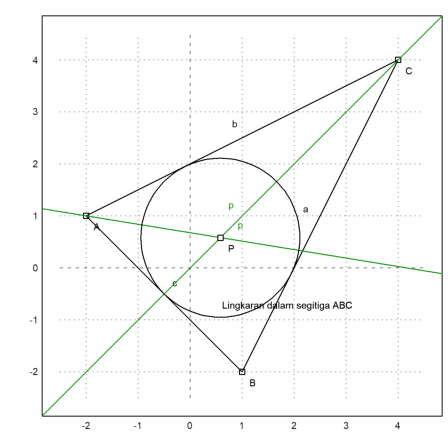
\includegraphics[keepaspectratio]{images/EMT4Geometry - Naila Khalidatus Salwa-013.png}}
\caption{images/EMT4Geometry\%20-\%20Naila\%20Khalidatus\%20Salwa-013.png}
\end{figure}

\begin{enumerate}
\def\labelenumi{\arabic{enumi}.}
\setcounter{enumi}{5}
\tightlist
\item
  Hitung luas lingkaran luar dan luas lingkaran dalam segitiga ABC. Adakah hubungan antara luas kedua lingkaran tersebut dengan luas segitiga ABC?
\end{enumerate}

Luas lingkaran luar

\textgreater C=pi*(R\^{}2)

\begin{verbatim}
4.36332312999
\end{verbatim}

Luas lingkaran dalam

\textgreater c=pi*(r\^{}2)

\begin{verbatim}
7.34417132895
\end{verbatim}

Luas segitiga ABC

\textgreater areaTriangle(A,B,C)

\begin{verbatim}
14.58996939
\end{verbatim}

Kesimpulan:

-Luas lingkaran dalam dan luar bergantung pada ukuran segitiga dan posisi titik pusat lingkaran.

\begin{itemize}
\tightlist
\item
  Tidak ada rumus tunggal yang menghubungkan ketiga luas tersebut secara langsung.
\end{itemize}

\chapter{Contoh 2: Geometri Simbolik}\label{contoh-2-geometri-simbolik}

Kita dapat menghitung geometri eksak dan simbolik menggunakan Maxima.

File geometri.e menyediakan fungsi yang sama (dan lebih banyak lagi) di Maxima. Namun, sekarang kita dapat menggunakan perhitungan simbolik.

\section{Menentukan persamaan garis yang melalui 2 titik}\label{menentukan-persamaan-garis-yang-melalui-2-titik}

\textgreater A \&= {[}1,0{]}; B \&= {[}0,1{]}; C \&= {[}2,2{]}; // menentukan tiga titik A, B, C

Fungsi garis dan lingkaran berfungsi sama seperti fungsi Euler, namun menyediakan komputasi simbolik.

\textgreater c \&= lineThrough(B,C) // c=BC

\begin{verbatim}
                             [- 1, 2, 2]
\end{verbatim}

\section{Mencari persamaan garis}\label{mencari-persamaan-garis}

Kita bisa mendapatkan persamaan garis dengan mudah.

\textgreater\$getLineEquation(c,x,y), \$solve(\%,y) \textbar{} expand // persamaan garis c

\[\left[ y=\frac{x}{2}+1 \right] \]\pandocbounded{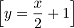
\includegraphics[keepaspectratio]{images/EMT4Geometry - Naila Khalidatus Salwa-015.png}}

\textgreater\$getLineEquation(lineThrough({[}x1,y1{]},{[}x2,y2{]}),x,y), \$solve(\%,y) // persamaan garis melalui(x1, y1) dan (x2, y2)

\[\left[ y=\frac{-\left({\it x_1}-x\right)\,{\it y_2}-\left(x-  {\it x_2}\right)\,{\it y_1}}{{\it x_2}-{\it x_1}} \right] \]\pandocbounded{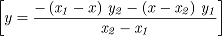
\includegraphics[keepaspectratio]{images/EMT4Geometry - Naila Khalidatus Salwa-017.png}}

\textgreater\$getLineEquation(lineThrough(A,{[}x1,y1{]}),x,y) // persamaan garis melalui A dan (x1, y1)

\[\left({\it x_1}-1\right)\,y-x\,{\it y_1}=-{\it y_1}\]Mencari garis yang tegak lurus BC dan melalui titik A

\textgreater h \&= perpendicular(A,lineThrough(B,C)) // h melalui A tegak lurus BC

\begin{verbatim}
                              [2, 1, 2]
\end{verbatim}

\section{Mencari titik potong garis h dengan garis BC}\label{mencari-titik-potong-garis-h-dengan-garis-bc}

\textgreater Q \&= lineIntersection(c,h) // Q titik potong garis c=BC dan h

\begin{verbatim}
                                 2  6
                                [-, -]
                                 5  5
\end{verbatim}

\textgreater\$projectToLine(A,lineThrough(B,C)) // proyeksi A pada BC

\[\left[ \frac{2}{5} , \frac{6}{5} \right] \]\#\# Mencari panjang garis AD

\textgreater\$distance(A,Q) // jarak AQ

\[\frac{3}{\sqrt{5}}\]\#\# Menentukan titik pusat dan jari-jari

\textgreater cc \&= circleThrough(A,B,C); \$cc // (titik pusat dan jari-jari) lingkaran melalui A, B, C

\[\left[ \frac{7}{6} , \frac{7}{6} , \frac{5}{3\,\sqrt{2}} \right] \]\textgreater r\&=getCircleRadius(cc); \$r , \$float(r) // tampilkan nilai jari-jari

\[1.178511301977579\]\pandocbounded{
\includegraphics[keepaspectratio]{images/EMT4Geometry - Naila Khalidatus Salwa-023.png}}

\section{Mencari nilai sudut ACB}\label{mencari-nilai-sudut-acb}

\textgreater\$computeAngle(A,C,B) // nilai \textless ACB

\[\arccos \left(\frac{4}{5}\right)\]\#\# Mencari persamaan garis bagi dan titik potong sudut ACB

\textgreater\$solve(getLineEquation(angleBisector(A,C,B),x,y),y){[}1{]} // persamaan garis bagi \textless ACB

\[y=x\]Mencari titik potong 2 garis tersebut

\textgreater P \&= lineIntersection(angleBisector(A,C,B),angleBisector(C,B,A)); \$P // titik potong 2 garis bagi sudut

\[\left[ \frac{\sqrt{2}\,\sqrt{5}+2}{6} , \frac{\sqrt{2}\,\sqrt{5}+2  }{6} \right] \]\textgreater P() // hasilnya sama dengan perhitungan sebelumnya

\begin{verbatim}
[0.86038,  0.86038]
\end{verbatim}

\section{Perpotongan Garis dan Lingkaran}\label{perpotongan-garis-dan-lingkaran}

Tentu saja, kita juga bisa memotong garis dengan lingkaran, dan lingkaran dengan lingkaran.

\textgreater A \&:= {[}1,0{]}; c=circleWithCenter(A,4);

\textgreater B \&:= {[}1,2{]}; C \&:= {[}2,1{]}; l=lineThrough(B,C);

\textgreater setPlotRange(5); plotCircle(c); plotLine(l,``l''); plotPoint(A,``A''); plotPoint (B,``B''), plotPoint (C,``C''):

\begin{figure}
\centering
\pandocbounded{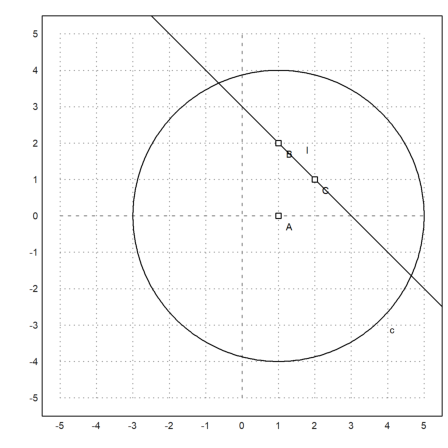
\includegraphics[keepaspectratio]{images/EMT4Geometry - Naila Khalidatus Salwa-027.png}}
\caption{images/EMT4Geometry\%20-\%20Naila\%20Khalidatus\%20Salwa-027.png}
\end{figure}

Perpotongan garis dengan lingkaran menghasilkan dua titik dan jumlah titik perpotongan.

\section{Mencari titik koordinat P1 dan P2 dalam (x,y)}\label{mencari-titik-koordinat-p1-dan-p2-dalam-xy}

\textgreater\{P1,P2,f\}=lineCircleIntersections(l,c);

\textgreater P1, P2, f

\begin{verbatim}
[4.64575,  -1.64575]
[-0.645751,  3.64575]
2
\end{verbatim}

\textgreater plotPoint(P1); plotPoint(P2):

\begin{figure}
\centering
\pandocbounded{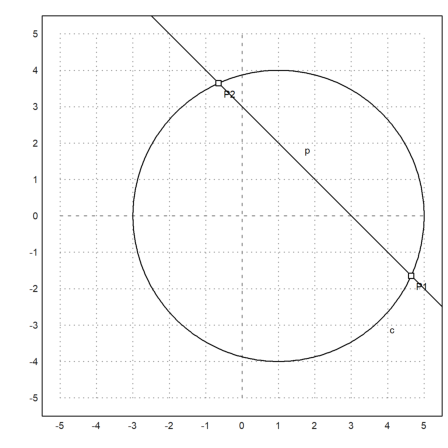
\includegraphics[keepaspectratio]{images/EMT4Geometry - Naila Khalidatus Salwa-028.png}}
\caption{images/EMT4Geometry\%20-\%20Naila\%20Khalidatus\%20Salwa-028.png}
\end{figure}

Hal yang sama di Maxima.

Menampilkan titik pusat dan jari-jari

\textgreater c \&= circleWithCenter(A,4) // lingkaran dengan pusat A jari-jari 4

\begin{verbatim}
                              [1, 0, 4]
\end{verbatim}

Menampilkan persamaan garis l yang melalui garis BC

\textgreater l \&= lineThrough(B,C) // garis l melalui B dan C

\begin{verbatim}
                              [1, 1, 3]
\end{verbatim}

Mencari titik potong antara sebuah garis l dan sebuah lingkaran c

\textgreater\$lineCircleIntersections(l,c) \textbar{} radcan, // titik potong lingkaran c dan garis l

\[\left[ \left[ \sqrt{7}+2 , 1-\sqrt{7} \right]  , \left[ 2-\sqrt{7}   , \sqrt{7}+1 \right]  \right] \]Akan ditunjukkan bahwa sudut-sudut yang menghadap bsuusr yang sama adalah sama besar.

\textgreater C=A+normalize({[}-2,-3{]})*4; plotPoint(C); plotSegment(P1,C); plotSegment(P2,C);

\textgreater degprint(computeAngle(P1,C,P2))

\begin{verbatim}
69°17'42.68''
\end{verbatim}

\textgreater C=A+normalize({[}-4,-3{]})*4; plotPoint(C); plotSegment(P1,C); plotSegment(P2,C);

\textgreater degprint(computeAngle(P1,C,P2))

\begin{verbatim}
69°17'42.68''
\end{verbatim}

\textgreater insimg;

\begin{figure}
\centering
\pandocbounded{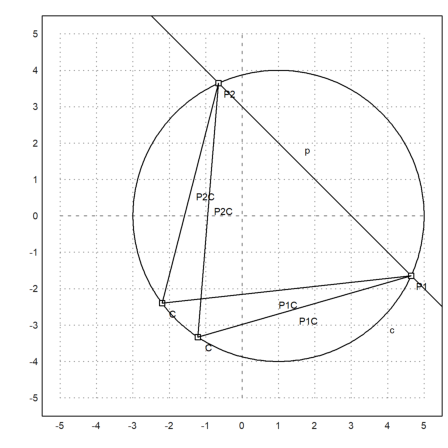
\includegraphics[keepaspectratio]{images/EMT4Geometry - Naila Khalidatus Salwa-030.png}}
\caption{images/EMT4Geometry\%20-\%20Naila\%20Khalidatus\%20Salwa-030.png}
\end{figure}

\section{Garis Sumbu}\label{garis-sumbu}

Berikut adalah langkah-langkah menggambar garis sumbu ruas garis AB:

\begin{enumerate}
\def\labelenumi{\arabic{enumi}.}
\item
  Gambar lingkaran dengan pusat A melalui B.
\item
  Gambar lingkaran dengan pusat B melalui A.
\item
  Tarik garis melallui kedua titik potong kedua lingkaran tersebut. Garis ini merupakan garis sumbu (melalui titik tengah dan tegak lurus) AB.
\end{enumerate}

Definisikan titik A dan titik B

\textgreater A={[}2,2{]}; B={[}-1,-2{]};

Membuat lingkaran C1 dan C2

\textgreater c1=circleWithCenter(A,distance(A,B));

\textgreater c2=circleWithCenter(B,distance(A,B));

\section{Mencari titik potong antara dua lingkaran}\label{mencari-titik-potong-antara-dua-lingkaran}

\textgreater\{P1,P2,f\}=circleCircleIntersections(c1,c2);

Garis yang melalui P1 dan P2

\textgreater l=lineThrough(P1,P2);

Mengatur rentang, titik, dan membuat plot lingkaran

\textgreater setPlotRange(5); plotCircle(c1); plotCircle(c2);

\textgreater plotPoint(A); plotPoint(B); plotSegment(A,B); plotLine(l):

\begin{figure}
\centering
\pandocbounded{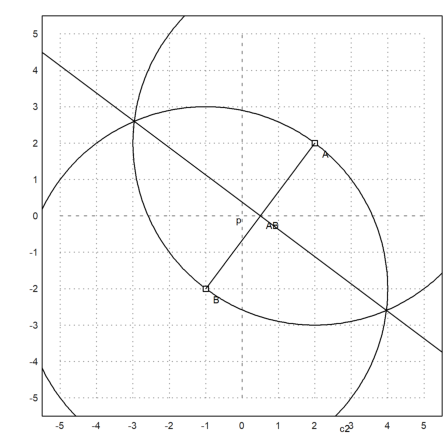
\includegraphics[keepaspectratio]{images/EMT4Geometry - Naila Khalidatus Salwa-031.png}}
\caption{images/EMT4Geometry\%20-\%20Naila\%20Khalidatus\%20Salwa-031.png}
\end{figure}

Selanjutnya kita melakukan hal yang sama di Maxima dengan koordinat umum.

Membuat lingkaran dan mencari titik potong

\textgreater A \&= {[}a1,a2{]}; B \&= {[}b1,b2{]};

\textgreater c1 \&= circleWithCenter(A,distance(A,B));

\textgreater c2 \&= circleWithCenter(B,distance(A,B));

\textgreater P \&= circleCircleIntersections(c1,c2); P1 \&= P{[}1{]}; P2 \&= P{[}2{]};

Persamaan untuk persimpangan cukup rumit. Tapi kita bisa menyederhanakannya jika kita mencari y.

\textgreater g \&= getLineEquation(lineThrough(P1,P2),x,y);

\textgreater\$solve(g,y)

\[\left[ y=\frac{-\left(2\,{\it b_1}-2\,{\it a_1}\right)\,x+{\it b_2}  ^2+{\it b_1}^2-{\it a_2}^2-{\it a_1}^2}{2\,{\it b_2}-2\,{\it a_2}}   \right] \]Persamaan ini biasanya berbentuk linear, y=mx+by dengan m sebagai gradien

Ini memang sama dengan garis tengah tegak lurus, yang dihitung dengan cara yang sangat berbeda.

\textgreater\$solve(getLineEquation(middlePerpendicular(A,B),x,y),y)

\[\left[ y=\frac{-\left(2\,{\it b_1}-2\,{\it a_1}\right)\,x+{\it b_2}  ^2+{\it b_1}^2-{\it a_2}^2-{\it a_1}^2}{2\,{\it b_2}-2\,{\it a_2}}   \right] \]Menentukan persamaan garis yang melalui titik A dan B:

\textgreater h \&=getLineEquation(lineThrough(A,B),x,y);

\textgreater\$solve(h,y)

\[\left[ y=\frac{\left({\it b_2}-{\it a_2}\right)\,x-{\it a_1}\,  {\it b_2}+{\it a_2}\,{\it b_1}}{{\it b_1}-{\it a_1}} \right] \]Perhatikan hasil kali gradien garis g dan h adalah:

\[\frac{-(b_1-a_1)}{(b_2-a_2)}\times \frac{(b_2-a_2)}{(b_1-a_1)} = -1.\]Artinya kedua garis tegak lurus.

\textgreater{}

\chapter{Contoh 3: Rumus Heron}\label{contoh-3-rumus-heron}

Rumus Heron menyatakan bahwa luas segitiga dengan panjang sisi-sisi a, b dan c adalah:

\[L = \sqrt{s(s-a)(s-b)(s-c)}\quad \text{ dengan } s=\frac{(a+b+c)}{2},\]atau bisa ditulis dalam bentuk lain:

\[L = \frac{1}{4}\sqrt{(a+b+c)(b+c-a)(a+c-b)(a+b-c)}\]Untuk membuktikan hal ini kita misalkan C(0,0), B(a,0) dan A(x,y), b=AC, c=AB. berikut visualisasi bentuk dari segitiga tersebut.

\textgreater setPlotRange(-1,10,-1,8); plotPoint({[}0,0{]}, ``C(0,0)''); plotPoint({[}5,0{]}, ``B(a,0)'');\ldots{}\\
\textgreater{} plotPoint({[}7,6{]}, ``A(x,y)'');

\textgreater plotSegment({[}0,0{]},{[}5.5,0{]}, ``a'',25); plotSegment({[}5.5,0{]},{[}7.5,6{]},``c'',15); \ldots{}\\
\textgreater{} plotSegment({[}0,0{]},{[}7.5,6{]},``b'',25);

\textgreater plotSegment({[}7.5,6{]},{[}7.5,0{]},``t=y'',25):

\begin{figure}
\centering
\pandocbounded{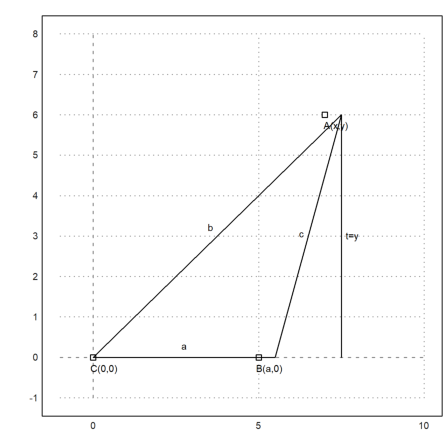
\includegraphics[keepaspectratio]{images/EMT4Geometry - Naila Khalidatus Salwa-038.png}}
\caption{images/EMT4Geometry\%20-\%20Naila\%20Khalidatus\%20Salwa-038.png}
\end{figure}

Luas segitiga ABC adalah

\[L_{\triangle ABC}=\frac{1}{2}a\times y.\]Nilai y didapat dari langkah-langkah berikut:

\[AC=\sqrt{(x-0)^2+(y-0)^2}\]\[b=\sqrt{x^2+y^2}\]\[b^2=x^2+y^2\]atau

\[AB=\sqrt{(x-a)^2+(y-0)^2}\]\[c=\sqrt{(x-a)^2+y^2}\]\[c^2=(x-a)^2+y^2\]kita akan memperoleh persamaan:

\[x^2+y^2=b^2\]

persamaan tersebut menyatakan bahwa titik (x,y) berjarak dari titik C(0,0)

\[(x-a)^2+y^2=c^2\]

persamaan tersebut menyatakan bahwa titik A(x,y) berjarak c dari titik B(a,0)

\textgreater\&assume(a\textgreater0); sol \&= solve({[}x\textsuperscript{2+y}2=b\textsuperscript{2,(x-a)}2+y\textsuperscript{2=c}2{]},{[}x,y{]})

\begin{verbatim}
                2    2    2
             - c  + b  + a
       [[x = --------------, y = 
                  2 a
          4      2  2      2  2    4      2  2    4
  sqrt(- c  + 2 b  c  + 2 a  c  - b  + 2 a  b  - a )
- --------------------------------------------------], 
                         2 a
        2    2    2
     - c  + b  + a
[x = --------------, y = 
          2 a
        4      2  2      2  2    4      2  2    4
sqrt(- c  + 2 b  c  + 2 a  c  - b  + 2 a  b  - a )
--------------------------------------------------]]
                       2 a
\end{verbatim}

Masukkan solusi dari y.

\textgreater ysol \&= y with sol{[}2{]}{[}2{]}; \$'y=sqrt(factor(ysol\^{}2))

\[y=\frac{\sqrt{\left(-c+b+a\right)\,\left(c-b+a\right)\,\left(c+b-a  \right)\,\left(c+b+a\right)}}{2\,a}\]Didapatkan rumus Heron.

\textgreater function H(a,b,c) \&= sqrt(factor((ysol*a/2)\^{}2)); \$'H(a,b,c)=H(a,b,c)

\[H\left(a , b , c\right)=\frac{\sqrt{\left(-c+b+a\right)\,\left(c-b+  a\right)\,\left(c+b-a\right)\,\left(c+b+a\right)}}{4}\]\textgreater\$'Luas=H(2,5,6) // luas segitiga dengan panjang sisi-sisi 2, 5, 6

\[{\it Luas}=\frac{3\,\sqrt{39}}{4}\]Tentu saja, setiap segitiga siku-siku adalah kasus yang terkenal.

\textgreater H(3,4,5) //luas segitiga siku-siku dengan panjang sisi 3, 4, 5

\begin{verbatim}
6
\end{verbatim}

Dan jelas juga bahwa ini adalah segitiga dengan luas maksimal dan kedua sisinya 3 dan 4.

\textgreater aspect (1.5); plot2d(\&H(3,4,x),1,7): // Kurva luas segitiga dengan panjang sisi 3, 4, x (1\textless= x \textless=7)

\begin{figure}
\centering
\pandocbounded{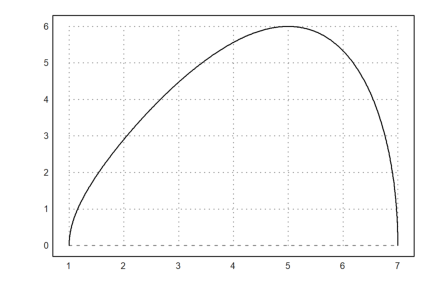
\includegraphics[keepaspectratio]{images/EMT4Geometry - Naila Khalidatus Salwa-051.png}}
\caption{images/EMT4Geometry\%20-\%20Naila\%20Khalidatus\%20Salwa-051.png}
\end{figure}

Kasus umum juga berhasil.

\section{Menggambar ellips dengan subtitusi}\label{menggambar-ellips-dengan-subtitusi}

\textgreater\$solve(diff(H(a,b,c)\^{}2,c)=0,c)

\[\left[ \frac{d}{d\,c}\,H\left(a , b , c\right)=0 , H\left(a , b , c  \right)=0 \right] \]Sekarang mari kita cari himpunan semua titik di mana b+c=d untuk suatu konstanta d.~Diketahui bahwa ini adalah elips.

\textgreater s1 \&= subst(d-c,b,sol{[}2{]}); \$s1

\[\left[ x=\frac{\left(d-c\right)^2-c^2+a^2}{2\,a} , y=\frac{\sqrt{-  \left(d-c\right)^4+2\,c^2\,\left(d-c\right)^2+2\,a^2\,\left(d-c  \right)^2-c^4+2\,a^2\,c^2-a^4}}{2\,a} \right] \]Buat suatu fungsi dari hasil subtitusi tersebut

\textgreater function fx(a,c,d) \&= rhs(s1{[}1{]}); \$fx(a,c,d), function fy(a,c,d) \&= rhs(s1{[}2{]}); \$fy(a,c,d)

\[\frac{\sqrt{-\left(d-c\right)^4+2\,c^2\,\left(d-c\right)^2+2\,a^2\,  \left(d-c\right)^2-c^4+2\,a^2\,c^2-a^4}}{2\,a}\]\pandocbounded{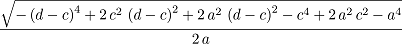
\includegraphics[keepaspectratio]{images/EMT4Geometry - Naila Khalidatus Salwa-055.png}}

Sekarang kita bisa menggambar plotnya. Ambil sisi b dengan rentang dari 1 sampai 4. Diketahui bahwa kita memperoleh elips.

\textgreater aspect(1); plot2d(\&fx(3,x,5),\&fy(3,x,5),xmin=1,xmax=4,square=1):

\begin{figure}
\centering
\pandocbounded{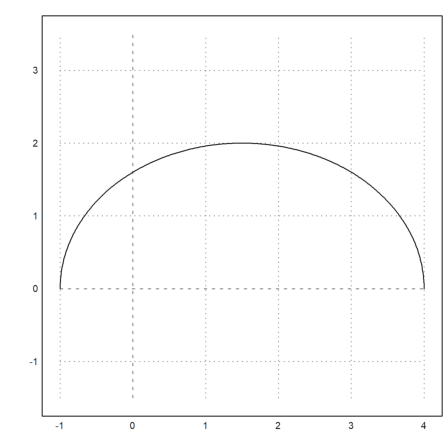
\includegraphics[keepaspectratio]{images/EMT4Geometry - Naila Khalidatus Salwa-056.png}}
\caption{images/EMT4Geometry\%20-\%20Naila\%20Khalidatus\%20Salwa-056.png}
\end{figure}

Kita dapat memeriksa persamaan umum elips ini, yaitu.

\[\frac{(x-x_m)^2}{u^2}+\frac{(y-y_m)}{v^2}=1,\]dimana (xm,ym) adalah pusat, dan u dan v adalah setengah sumbu.

\textgreater\$ratsimp((fx(a,c,d)-a/2)\textsuperscript{2/u}2+fy(a,c,d)\textsuperscript{2/v}2 with {[}u=d/2,v=sqrt(d\textsuperscript{2-a}2)/2{]})

\[1\]Kita melihat bahwa tinggi dan luas segitiga adalah maksimal untuk x=0. Jadi luas segitiga dengan a+b+c=d adalah maksimal jika segitiga tersebut sama sisi. Kami ingin memperolehnya secara analitis.

\textgreater eqns \&= {[}diff(H(a,b,d-(a+b))\textsuperscript{2,a)=0,diff(H(a,b,d-(a+b))}2,b)=0{]}; \$eqns

\[\left[ \frac{d\,\left(d-2\,a\right)\,\left(d-2\,b\right)}{8}-\frac{  \left(-d+2\,b+2\,a\right)\,d\,\left(d-2\,b\right)}{8}=0 , \frac{d\,  \left(d-2\,a\right)\,\left(d-2\,b\right)}{8}-\frac{\left(-d+2\,b+2\,  a\right)\,d\,\left(d-2\,a\right)}{8}=0 \right] \]Kita mendapatkan nilai minimum yang dimiliki oleh segitiga dengan salah satu sisinya 0, dan solusinya a=b=c=d/3.

\textgreater\$solve(eqns,{[}a,b{]})

\[\left[ \left[ a=\frac{d}{3} , b=\frac{d}{3} \right]  , \left[ a=0   , b=\frac{d}{2} \right]  , \left[ a=\frac{d}{2} , b=0 \right]  ,   \left[ a=\frac{d}{2} , b=\frac{d}{2} \right]  \right] \]Ada juga metode Lagrange, yang memaksimalkan H(a,b,c)\^{}2 terhadap a+b+d=d.

\textgreater\&solve({[}diff(H(a,b,c)\textsuperscript{2,a)=la,diff(H(a,b,c)}2,b)=la, \ldots{}\\
\textgreater{} diff(H(a,b,c)\^{}2,c)=la,a+b+c=d{]},{[}a,b,c,la{]})

\begin{verbatim}
                    d      d                d             d
       [[a = 0, b = -, c = -, la = 0], [a = -, b = 0, c = -, la = 0], 
                    2      2                2             2
                                                                  3
            d      d                       d      d      d       d
       [a = -, b = -, c = 0, la = 0], [a = -, b = -, c = -, la = ---]]
            2      2                       3      3      3       108
\end{verbatim}

Kita bisa membuat plot situasinya

Pertama atur titik di Maxima.

\textgreater A \&= at({[}x,y{]},sol{[}2{]}); \$A

\[\left[ \frac{-c^2+b^2+a^2}{2\,a} , \frac{\sqrt{-c^4+2\,b^2\,c^2+2\,  a^2\,c^2-b^4+2\,a^2\,b^2-a^4}}{2\,a} \right] \]\textgreater B \&= {[}0,0{]}; \$B, C \&= {[}a,0{]}; \$C

\[\left[ a , 0 \right] \]\pandocbounded{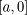
\includegraphics[keepaspectratio]{images/EMT4Geometry - Naila Khalidatus Salwa-063.png}}

Kemudian atur rentang plot, dan plot titik-titiknya.

\textgreater setPlotRange(0,5,-2,3); \ldots{}\\
\textgreater{} a=4; b=3; c=2; \ldots{}\\
\textgreater{} plotPoint(mxmeval(``B''),``B''); plotPoint(mxmeval(``C''),``C''); \ldots{}\\
\textgreater{} plotPoint(mxmeval(``A''),``A''):

\begin{figure}
\centering
\pandocbounded{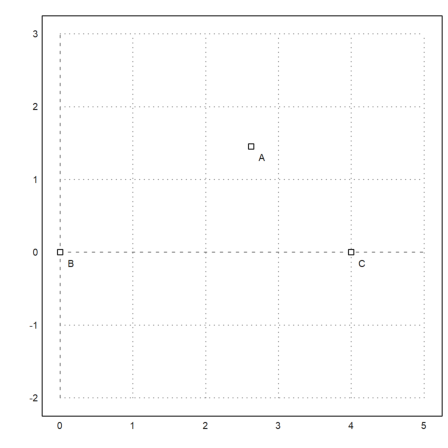
\includegraphics[keepaspectratio]{images/EMT4Geometry - Naila Khalidatus Salwa-064.png}}
\caption{images/EMT4Geometry\%20-\%20Naila\%20Khalidatus\%20Salwa-064.png}
\end{figure}

Plot segmennya.

\textgreater plotSegment(mxmeval(``A''),mxmeval(``C'')); \ldots{}\\
\textgreater{} plotSegment(mxmeval(``B''),mxmeval(``C'')); \ldots{}\\
\textgreater{} plotSegment(mxmeval(``B''),mxmeval(``A'')):

\begin{figure}
\centering
\pandocbounded{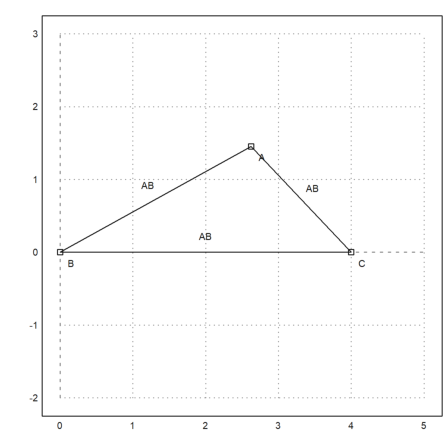
\includegraphics[keepaspectratio]{images/EMT4Geometry - Naila Khalidatus Salwa-065.png}}
\caption{images/EMT4Geometry\%20-\%20Naila\%20Khalidatus\%20Salwa-065.png}
\end{figure}

Hitung garis tengah tegak lurus di Maxima.

\textgreater h \&= middlePerpendicular(A,B); g \&= middlePerpendicular(B,C);

Dan pusat lingkarannya.

\textgreater U \&= lineIntersection(h,g);

Kita mendapatkan rumus jari-jari lingkaran luar.

\textgreater\&assume(a\textgreater0,b\textgreater0,c\textgreater0); \$distance(U,B) \textbar{} radcan

\[\frac{i\,a\,b\,c}{\sqrt{c-b-a}\,\sqrt{c-b+a}\,\sqrt{c+b-a}\,\sqrt{c  +b+a}}\]Mari kita tambahkan ini ke dalam plot.

\textgreater plotPoint(U()); \ldots{}\\
\textgreater{} plotCircle(circleWithCenter(mxmeval(``U''),mxmeval(``distance(U,C)''))):

\begin{figure}
\centering
\pandocbounded{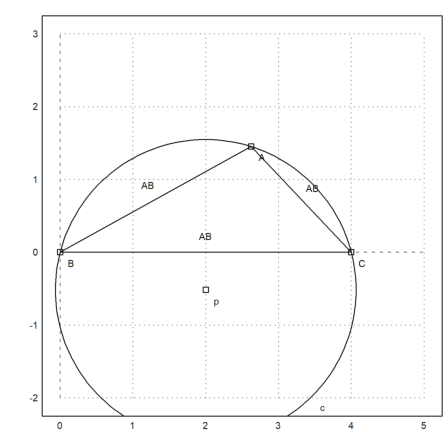
\includegraphics[keepaspectratio]{images/EMT4Geometry - Naila Khalidatus Salwa-067.png}}
\caption{images/EMT4Geometry\%20-\%20Naila\%20Khalidatus\%20Salwa-067.png}
\end{figure}

Dengan menggunakan geometri, kita memperoleh rumus sederhana

\[\frac{a}{\sin(\alpha)}=2r\]untuk radius. Kita bisa cek, apakah ini benar adanya pada Maxima. Maxima akan memfaktorkan ini hanya jika kita mengkuadratkannya.

\textgreater\$c\textsuperscript{2/sin(computeAngle(A,B,C))}2 \textbar{} factor

\[-\frac{4\,a^2\,b^2\,c^2}{\left(c-b-a\right)\,\left(c-b+a\right)\,  \left(c+b-a\right)\,\left(c+b+a\right)}\]\# Contoh 4: Garis Euler dan Parabola

Garis Euler adalah garis yang ditentukan dari sembarang segitiga yang tidak sama sisi. Merupakan garis tengah segitiga, dan melewati beberapa titik penting yang ditentukan dari segitiga, antara lain orthocenter, circumcenter, centroid, titik Exeter dan pusat lingkaran sembilan titik segitiga.

orthocenter : titik perpotongan garis tinggi

circumcenter : titik pusat lingkaran luar segitiga

centroid : titik berat atau pusat massa segitiga

titik Exeter : titik istimewa yang terletak pada sumbu Euler

Untuk demonstrasinya, kita menghitung dan memplot garis Euler dalam sebuah segitiga.

Pertama, kita mendefinisikan sudut-sudut segitiga di Euler. Kami menggunakan definisi, yang terlihat dalam ekspresi simbolik.

\textgreater A::={[}-1,-1{]}; B::={[}2,0{]}; C::={[}1,2{]};

Untuk memplot objek geometris, kita menyiapkan area plot, dan menambahkan titik ke dalamnya. Semua plot objek geometris ditambahkan ke plot saat ini.

\textgreater setPlotRange(3); plotPoint(A,``A''); plotPoint(B,``B''); plotPoint(C,``C'');

Kita juga bisa menjumlahkan sisi-sisi segitiga.

\textgreater plotSegment(A,B,``\,``); plotSegment(B,C,''``); plotSegment(C,A,''\,``):

\begin{figure}
\centering
\pandocbounded{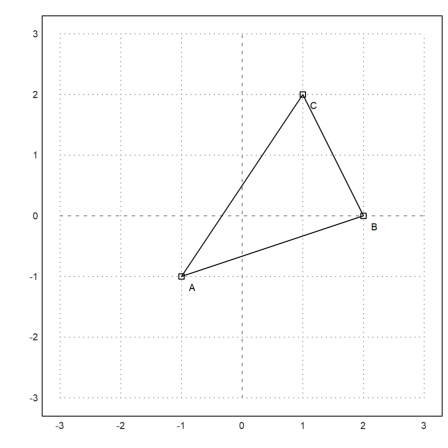
\includegraphics[keepaspectratio]{images/EMT4Geometry - Naila Khalidatus Salwa-070.png}}
\caption{images/EMT4Geometry\%20-\%20Naila\%20Khalidatus\%20Salwa-070.png}
\end{figure}

Berikut luas segitiga menggunakan rumus determinan. Tentu saja kami harus mengambil nilai absolut dari hasil ini.

\textgreater\$areaTriangle(A,B,C)

\[-\frac{7}{2}\]Kita dapat menghitung koefisien sisi c.

\textgreater c \&= lineThrough(A,B)

\begin{verbatim}
                            [- 1, 3, - 2]
\end{verbatim}

Dan dapatkan juga rumus untuk baris ini.

\textgreater\$getLineEquation(c,x,y)

\[3\,y-x=-2\]Untuk bentuk Hesse, kita perlu menentukan sebuah titik, sehingga titik tersebut berada di sisi positif dari Hesseform. Memasukkan titik akan menghasilkan jarak positif ke garis.

\textgreater\$getHesseForm(c,x,y,C), \$at(\%,{[}x=C{[}1{]},y=C{[}2{]}{]})

\[\frac{7}{\sqrt{10}}\]\pandocbounded{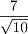
\includegraphics[keepaspectratio]{images/EMT4Geometry - Naila Khalidatus Salwa-074.png}}

\section{Lingkaran luar dan lingkaran dalam}\label{lingkaran-luar-dan-lingkaran-dalam}

Sekarang kita menghitung lingkaran luar ABC.

\textgreater LL \&= circleThrough(A,B,C); \$getCircleEquation(LL,x,y)

\[\left(y-\frac{5}{14}\right)^2+\left(x-\frac{3}{14}\right)^2=\frac{  325}{98}\]\textgreater O \&= getCircleCenter(LL); \$O

\[\left[ \frac{3}{14} , \frac{5}{14} \right] \]Plot lingkaran dan pusatnya. Cu dan U bersifat simbolis. Kami mengevaluasi ekspresi ini untuk Euler.

\textgreater plotCircle(LL()); plotPoint(O(),``O''):

\begin{figure}
\centering
\pandocbounded{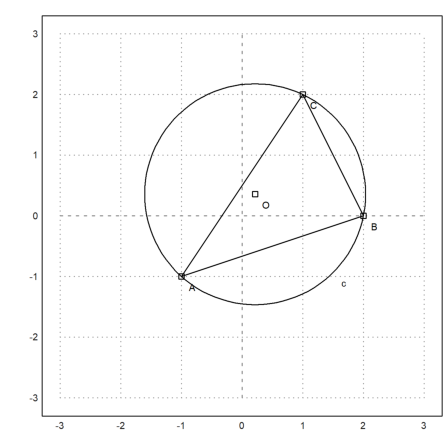
\includegraphics[keepaspectratio]{images/EMT4Geometry - Naila Khalidatus Salwa-077.png}}
\caption{images/EMT4Geometry\%20-\%20Naila\%20Khalidatus\%20Salwa-077.png}
\end{figure}

Kita dapat menghitung perpotongan ketinggian di ABC (ortocenter) secara numerik dengan perintah berikut.

\textgreater H \&= lineIntersection(perpendicular(A,lineThrough(C,B)),\ldots{}\\
\textgreater{} perpendicular(B,lineThrough(A,C))); \$H

\[\left[ \frac{11}{7} , \frac{2}{7} \right] \]Sekarang kita dapat menghitung garis segitiga Euler.

\textgreater el \&= lineThrough(H,O); \$getLineEquation(el,x,y)

\[-\frac{19\,y}{14}-\frac{x}{14}=-\frac{1}{2}\]Tambahkan ini ke plot.

\textgreater plotPoint(H(),``H''); plotLine(el(),``Garis Euler''):

\begin{figure}
\centering
\pandocbounded{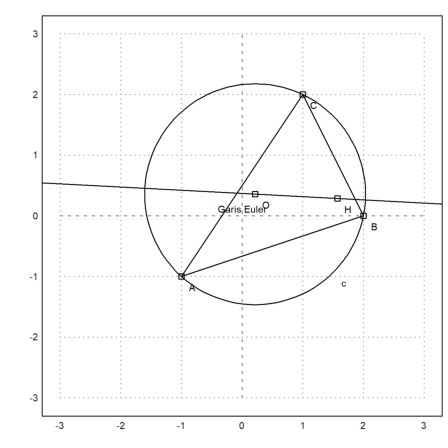
\includegraphics[keepaspectratio]{images/EMT4Geometry - Naila Khalidatus Salwa-080.png}}
\caption{images/EMT4Geometry\%20-\%20Naila\%20Khalidatus\%20Salwa-080.png}
\end{figure}

Pusat gravitasi seharusnya berada di garis ini.

\textgreater M \&= (A+B+C)/3; \$getLineEquation(el,x,y) with

\[-\frac{1}{2}=-\frac{1}{2}\]\textgreater plotPoint(M(),``M''): // titik berat

\begin{figure}
\centering
\pandocbounded{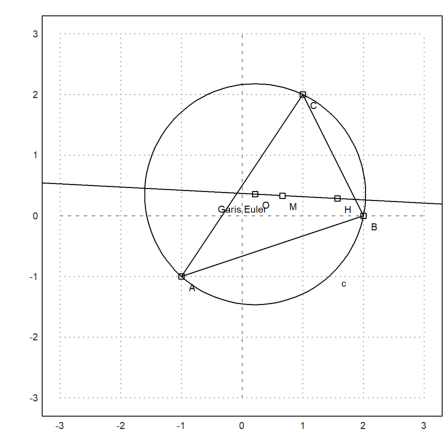
\includegraphics[keepaspectratio]{images/EMT4Geometry - Naila Khalidatus Salwa-082.png}}
\caption{images/EMT4Geometry\%20-\%20Naila\%20Khalidatus\%20Salwa-082.png}
\end{figure}

Teorinya memberitahu kita MH=2*MO. Kita perlu menyederhanakan dengan radcan untuk mencapai hal ini.

\textgreater\$distance(M,H)/distance(M,O)\textbar radcan

\[2\]Fungsinya mencakup fungsi untuk sudut juga.

\textgreater\$computeAngle(A,C,B), degprint(\%())

\[\arccos \left(\frac{4}{\sqrt{5}\,\sqrt{13}}\right)\] 60°15'18.43'\,'

Persamaan pusat lingkaran tidak terlalu bagus.

\textgreater Q \&= lineIntersection(angleBisector(A,C,B),angleBisector(C,B,A))\textbar radcan; \$Q

\[\left[ \frac{\left(2^{\frac{3}{2}}+1\right)\,\sqrt{5}\,\sqrt{13}-15  \,\sqrt{2}+3}{14} , \frac{\left(\sqrt{2}-3\right)\,\sqrt{5}\,\sqrt{  13}+5\,2^{\frac{3}{2}}+5}{14} \right] \]Mari kita hitung juga ekspresi jari-jari lingkaran yang tertulis.

\textgreater r \&= distance(Q,projectToLine(Q,lineThrough(A,B)))\textbar ratsimp; \$r

\[\frac{\sqrt{\left(-41\,\sqrt{2}-31\right)\,\sqrt{5}\,\sqrt{13}+115  \,\sqrt{2}+614}}{7\,\sqrt{2}}\]\textgreater LD \&= circleWithCenter(Q,r); // Lingkaran dalam

Mari kita tambahkan ini ke dalam plot.

\textgreater color(5); plotCircle(LD()):

\begin{figure}
\centering
\pandocbounded{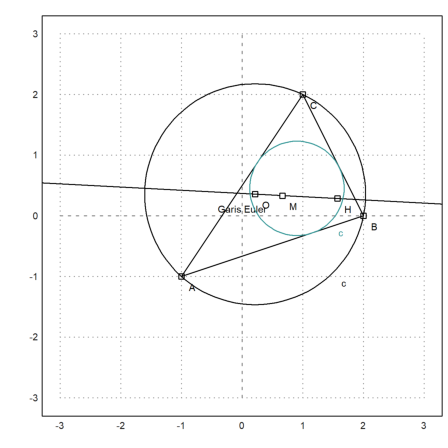
\includegraphics[keepaspectratio]{images/EMT4Geometry - Naila Khalidatus Salwa-087.png}}
\caption{images/EMT4Geometry\%20-\%20Naila\%20Khalidatus\%20Salwa-087.png}
\end{figure}

\section{Parabola}\label{parabola}

Selanjutnya akan dicari persamaan tempat kedudukan titik-titik yang berjarak sama ke titik C dan ke garis AB.

\textgreater p \&= getHesseForm(lineThrough(A,B),x,y,C)-distance({[}x,y{]},C); \$p='0

\[\frac{3\,y-x+2}{\sqrt{10}}-\sqrt{\left(2-y\right)^2+\left(1-x  \right)^2}=0\]Persamaan tersebut dapat digambar menjadi satu dengan gambar sebelumnya.

\textgreater plot2d(p,level=0,add=1,contourcolor=6):

\begin{figure}
\centering
\pandocbounded{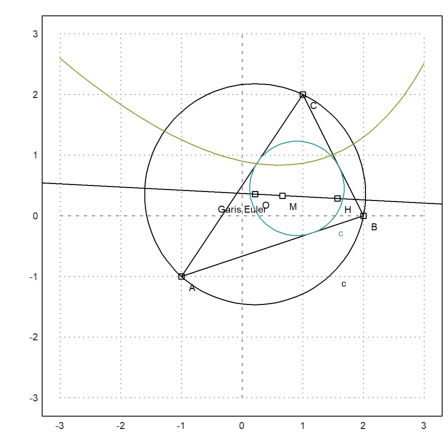
\includegraphics[keepaspectratio]{images/EMT4Geometry - Naila Khalidatus Salwa-089.png}}
\caption{images/EMT4Geometry\%20-\%20Naila\%20Khalidatus\%20Salwa-089.png}
\end{figure}

Ini seharusnya merupakan suatu fungsi, tetapi pemecah default Maxima hanya dapat menemukan solusinya, jika kita mengkuadratkan persamaannya. Akibatnya, kita mendapatkan solusi palsu.

\textgreater akar \&= solve(getHesseForm(lineThrough(A,B),x,y,C)\textsuperscript{2-distance({[}x,y{]},C)}2,y)

\begin{verbatim}
        [y = - 3 x - sqrt(70) sqrt(9 - 2 x) + 26, 
                              y = - 3 x + sqrt(70) sqrt(9 - 2 x) + 26]
\end{verbatim}

Solusi pertama adalah

\[{\it akar}_{1}\]Menambahkan solusi pertama pada plot menunjukkan, bahwa itu memang jalan yang kita cari. Teorinya memberitahu kita bahwa itu adalah parabola yang diputar.

\textgreater plot2d(\&rhs(akar{[}1{]}),add=1):

\begin{figure}
\centering
\pandocbounded{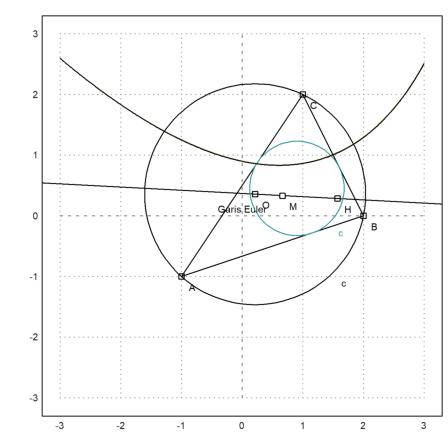
\includegraphics[keepaspectratio]{images/EMT4Geometry - Naila Khalidatus Salwa-091.png}}
\caption{images/EMT4Geometry\%20-\%20Naila\%20Khalidatus\%20Salwa-091.png}
\end{figure}

\textgreater function g(x) \&= rhs(akar{[}1{]}); \$'g(x)= g(x)// fungsi yang mendefinisikan kurva di atas

\[g\left(x\right)=-3\,x-\sqrt{70}\,\sqrt{9-2\,x}+26\]\textgreater T \&={[}-1, g(-1){]}; // ambil sebarang titik pada kurva tersebut

\textgreater dTC \&= distance(T,C); \$fullratsimp(dTC), \$float(\%) // jarak T ke C

\[2.135605779339061\]\pandocbounded{
\includegraphics[keepaspectratio]{images/EMT4Geometry - Naila Khalidatus Salwa-094.png}}

\textgreater U \&= projectToLine(T,lineThrough(A,B)); \$U // proyeksi T pada garis AB

\[\left[ \frac{80-3\,\sqrt{11}\,\sqrt{70}}{10} , \frac{20-\sqrt{11}\,  \sqrt{70}}{10} \right] \]\textgreater dU2AB \&= distance(T,U); \$fullratsimp(dU2AB), \$float(\%) // jatak T ke AB

\[2.135605779339061\]\pandocbounded{
\includegraphics[keepaspectratio]{images/EMT4Geometry - Naila Khalidatus Salwa-097.png}}

Kesimpulan: jarak T ke C sama dengan jarak T ke AB. Perhitungan ini menunjukkan bahwa proyeksi titik T pada garis AB menghasilkan jarak yang sama dengan jarak langsung antara T dan C, sehingga memperlihatkan bahwa titik C terletak pada garis AB.

\chapter{Contoh 5: Trigonometri Rasional}\label{contoh-5-trigonometri-rasional}

Hal ini terinspirasi dari ceramah N.J.Wildberger. Dalam bukunya ``Divine Proportions'', Wildberger mengusulkan untuk mengganti gagasan klasik tentang jarak dan sudut dengan kuadran dan penyebaran. Dengan menggunakan hal ini, memang mungkin untuk menghindari fungsi trigonometri dalam banyak contoh, dan tetap ``rasional''.

Berikut ini, saya memperkenalkan konsep, dan memecahkan beberapa masalah. Saya menggunakan perhitungan simbolik Maxima di sini, yang menyembunyikan keunggulan utama trigonometri rasional yaitu perhitungan hanya dapat dilakukan dengan kertas dan pensil. Anda diundang untuk memeriksa hasilnya tanpa komputer.

Intinya adalah perhitungan rasional simbolik seringkali memberikan hasil yang sederhana. Sebaliknya, trigonometri klasik menghasilkan hasil trigonometri yang rumit, yang hanya mengevaluasi perkiraan numerik saja.

\textgreater load geometry;

Untuk pengenalan pertama, kami menggunakan segitiga siku-siku dengan proporsi Mesir yang terkenal 3, 4 dan 5. Perintah berikut adalah perintah Euler untuk memplot geometri bidang yang terdapat dalam file Euler ``geometry.e''.

\textgreater C\&:={[}0,0{]}; A\&:={[}4,0{]}; B\&:={[}0,3{]}; \ldots{}\\
\textgreater{} setPlotRange(-1,5,-1,5); \ldots{}\\
\textgreater{} plotPoint(A,``A''); plotPoint(B,``B''); plotPoint(C,``C''); \ldots{}\\
\textgreater{} plotSegment(B,A,``c''); plotSegment(A,C,``b''); plotSegment(C,B,``a''); \ldots{}\\
\textgreater{} insimg(30);

\begin{figure}
\centering
\pandocbounded{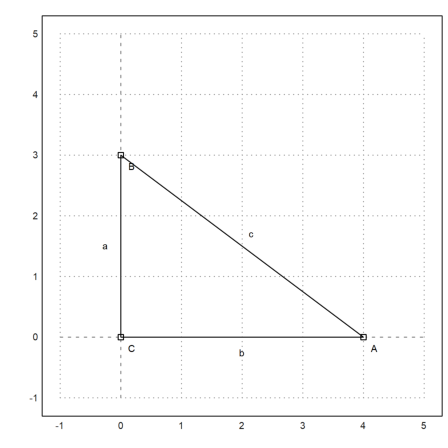
\includegraphics[keepaspectratio]{images/EMT4Geometry - Naila Khalidatus Salwa-098.png}}
\caption{images/EMT4Geometry\%20-\%20Naila\%20Khalidatus\%20Salwa-098.png}
\end{figure}

Tentu saja,

\[\sin(w_a)=\frac{a}{c},\]dimana wa adalah sudut di A. Cara umum untuk menghitung sudut ini adalah dengan mengambil invers dari fungsi sinus. Hasilnya adalah sudut yang tidak dapat dicerna, yang hanya dapat dicetak secara kasar.

\textgreater wa := arcsin(3/5); degprint(wa)

\begin{verbatim}
36°52'11.63''
\end{verbatim}

Trigonometri rasional mencoba menghindari hal ini.

Gagasan pertama tentang trigonometri rasional adalah kuadran, yang menggantikan jarak. Faktanya, itu hanyalah jarak yang dikuadratkan. Di bawah ini, a, b, dan c menyatakan kuadran sisi-sisinya.

Teorema Pythogoras menjadi a+b=c.

\[a+b=c\]\[(3^2)+(4^2)=5^2\]\[9+16=25\]\[25=25\]\textgreater a \&= 3\^{}2; b \&= 4\^{}2; c \&= 5\^{}2; \&a+b=c

\begin{verbatim}
                               25 = 25
\end{verbatim}

Pengertian trigonometri rasional yang kedua adalah penyebaran. Penyebaran mengukur pembukaan antar garis. Nilainya 0 jika garisnya sejajar, dan 1 jika garisnya persegi panjang. Ini adalah kuadrat sinus sudut antara dua garis.

Luas garis AB dan AC pada gambar di atas didefinisikan sebagai

\[s_a = \sin(\alpha)^2 = \frac{a}{c},\]dimana a dan c adalah kuadran suatu segitiga siku-siku yang salah satu sudutnya berada di A.

\textgreater sa \&= a/c; \$sa

\[\frac{9}{25}\]Tentu saja ini lebih mudah dihitung daripada sudutnya. Namun Anda kehilangan properti bahwa sudut dapat ditambahkan dengan mudah.

Tentu saja, kita dapat mengonversi nilai perkiraan sudut wa menjadi sprad, dan mencetaknya sebagai pecahan.

\textgreater fracprint(sin(wa)\^{}2)

\begin{verbatim}
9/25
\end{verbatim}

Hukum kosinus trigonometri klasik diterjemahkan menjadi ``hukum silang'' berikut.

\[(c+b-a)^2 = 4 b c \, (1-s_a)\]Di sini a, b, dan c adalah kuadran sisi-sisi segitiga, dan sa adalah jarak di sudut A. Sisi a, seperti biasa, berhadapan dengan sudut A.

Hukum-hukum ini diterapkan dalam file geometry.e yang kami muat ke Euler.

\textgreater\$crosslaw(aa,bb,cc,saa)

\[\left({\it cc}+{\it bb}-{\it aa}\right)^2=4\,{\it bb}\,{\it cc}\,  \left(1-{\it saa}\right)\]Dalam kasus kita, didapatkan

\textgreater\$crosslaw(a,b,c,sa)

\[1024=1024\]Mari kita gunakan hukum silang ini untuk mencari penyebaran di A. Untuk melakukannya, kita buat hukum silang untuk kuadran a, b, dan c, dan selesaikan untuk penyebaran yang tidak diketahui sa.

Anda bisa melakukannya dengan tangan dengan mudah, tapi saya menggunakan Maxima. Tentu saja, kami mendapatkan hasilnya, kami sudah mendapatkannya.

\textgreater\$crosslaw(a,b,c,x), \$solve(\%,x)

\[\left[ x=\frac{9}{25} \right] \]\pandocbounded{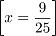
\includegraphics[keepaspectratio]{images/EMT4Geometry - Naila Khalidatus Salwa-110.png}}

Kita sudah mengetahui hal ini. Definisi penyebaran adalah kasus khusus dari crosslaw. Kita juga dapat menyelesaikannya untuk a, b, c secara umum. Hasilnya adalah sebuah rumus yang menghitung penyebaran sudut sebuah segitiga dengan kuadran ketiga sisinya.

\textgreater\$solve(crosslaw(aa,bb,cc,x),x)

\[\left[ x=\frac{-{\it cc}^2-\left(-2\,{\it bb}-2\,{\it aa}\right)\,  {\it cc}-{\it bb}^2+2\,{\it aa}\,{\it bb}-{\it aa}^2}{4\,{\it bb}\,  {\it cc}} \right] \]Kita bisa membuat fungsi dari hasilnya. Fungsi seperti itu sudah didefinisikan dalam file geometry.e dari Euler.

\textgreater\$spread(a,b,c)

\[\frac{9}{25}\]Sebagai contoh, kita dapat menggunakannya untuk menghitung sudut segitiga dengan sisi-sisi

\[a, \quad a, \quad \frac{4a}{7}\]Hasilnya adalah rasional, yang tidak mudah didapat jika kita menggunakan trigonometri klasik.

\textgreater\$spread(a,a,4*a/7)

Ini adalah sudut dalam derajat.

\textgreater degprint(arcsin(sqrt(6/7)))

\begin{verbatim}
67°47'32.44''
\end{verbatim}

\section{Contoh Lain}\label{contoh-lain}

Sekarang, mari kita coba contoh yang lebih maju. Kita tentukan tiga sudut segitiga sebagai berikut.

\textgreater A\&:={[}1,2{]}; B\&:={[}4,3{]}; C\&:={[}0,4{]}; \ldots{}\\
\textgreater{} setPlotRange(-1,5,1,7); \ldots{}\\
\textgreater{} plotPoint(A,``A''); plotPoint(B,``B''); plotPoint(C,``C''); \ldots{}\\
\textgreater{} plotSegment(B,A,``c''); plotSegment(A,C,``b''); plotSegment(C,B,``a''); \ldots{}\\
\textgreater{} insimg;

\begin{figure}
\centering
\pandocbounded{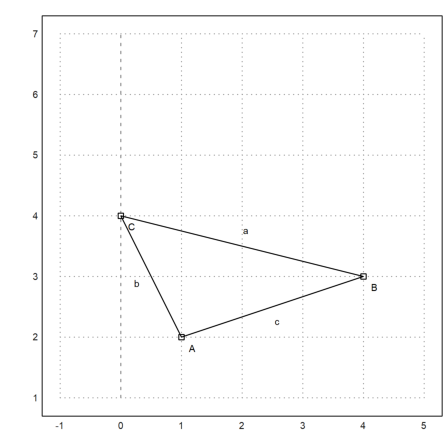
\includegraphics[keepaspectratio]{images/EMT4Geometry - Naila Khalidatus Salwa-114.png}}
\caption{images/EMT4Geometry\%20-\%20Naila\%20Khalidatus\%20Salwa-114.png}
\end{figure}

Dengan menggunakan Pythogoras, mudah untuk menghitung jarak antara dua titik. Pertama-tama saya menggunakan fungsi jarak dari file Euler untuk geometri. Jarak fungsi menggunakan geometri klasik.

\textgreater\$distance(A,B)

\[\sqrt{10}\]Euler juga memiliki fungsi untuk kuadransi antara dua titik.

Pada contoh berikut, karena c+b bukan a, maka segitiga tersebut tidak berbentuk persegi panjang.

\textgreater c \&= quad(A,B); \$c, b \&= quad(A,C); \$b, a \&= quad(B,C); \$a,

\[17\]\pandocbounded{
\includegraphics[keepaspectratio]{images/EMT4Geometry - Naila Khalidatus Salwa-117.png}}

\begin{figure}
\centering
\pandocbounded{
\includegraphics[keepaspectratio]{images/EMT4Geometry - Naila Khalidatus Salwa-118.png}}
\caption{images/EMT4Geometry\%20-\%20Naila\%20Khalidatus\%20Salwa-118.png}
\end{figure}

Pertama, mari kita menghitung sudut tradisional. Fungsi computeAngle menggunakan metode yang biasa berdasarkan hasil kali titik dari dua vektor. Hasilnya adalah beberapa perkiraan titik mengambang

\[A=<1,2>\quad B=<4,3>,\quad C=<0,4>\]\[\mathbf{a}=C-B=<-4,1>,\quad \mathbf{c}=A-B=<-3,-1>,\quad \beta=\angle ABC\]\[\mathbf{a}.\mathbf{c}=|\mathbf{a}|.|\mathbf{c}|\cos \beta\]\[\cos \angle ABC =\cos\beta=\frac{\mathbf{a}.\mathbf{c}}{|\mathbf{a}|.|\mathbf{c}|}=\frac{12-1}{\sqrt{17}\sqrt{10}}=\frac{11}{\sqrt{17}\sqrt{10}}\]\textgreater wb \&= computeAngle(A,B,C); \$wb, \$(wb/pi*180)()

\[\arccos \left(\frac{11}{\sqrt{10}\,\sqrt{17}}\right)\] 32.4711922908

Dengan menggunakan pensil dan kertas, kita bisa melakukan hal yang sama dengan hukum silang. Kita masukkan kuadran a, b, dan c ke dalam hukum silang dan selesaikan untuk x.

\textgreater\$crosslaw(a,b,c,x), \$solve(\%,x), //(b+c-a)\^{}=4b.c(1-x)

\[\left[ x=\frac{9}{25} \right] \]\pandocbounded{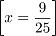
\includegraphics[keepaspectratio]{images/EMT4Geometry - Naila Khalidatus Salwa-125.png}}

Itulah yang dilakukan oleh fungsi spread yang didefinisikan dalam ``geometry.e''.

\textgreater sb \&= spread(b,a,c); \$sb

\[\frac{16}{25}\]Maxima mendapatkan hasil yang sama dengan menggunakan trigonometri biasa, jika kita memaksakannya. Ia menyelesaikan suku sin(arccos(\ldots)) menjadi hasil pecahan. Sebagian besar siswa tidak dapat melakukan ini.

\textgreater\$sin(computeAngle(A,B,C))\^{}2

\[\frac{49}{170}\]Setelah kita memiliki penyebaran di B, kita dapat menghitung tinggi ha di sisi a. Ingatlah bahwa

\[s_b = \frac{h_a}{c} \]

menurut definisi.

\textgreater ha \&= c*sb; \$ha

\[16\]Gambar berikut ini dibuat dengan program geometri C.a.R., yang dapat menggambar kuadran dan sebaran.

image: (20) Rational\_Geometry\_CaR.png

Secara definisi, panjang ha adalah akar kuadrat dari kuadran.

\textgreater\$sqrt(ha)

\[4\]Sekarang kita bisa menghitung luas segitiga. Jangan lupa, bahwa kita berurusan dengan kuadran!

\textgreater\$sqrt(ha)*sqrt(a)/2

\[6\]Rumus penentu yang biasa menghasilkan hasil yang sama.

\textgreater\$areaTriangle(B,A,C)

\[\frac{7}{2}\]\#\# Rumus Heron

Sekarang, mari kita selesaikan masalah ini secara umum!

\textgreater\&remvalue(a,b,c,sb,ha);

Pertama-tama kita menghitung luas di B untuk segitiga dengan sisi a, b, dan c.~Kemudian kita menghitung luas kuadrat (``quadrea''?), memfaktorkannya dengan Maxima, dan kita mendapatkan rumus Heron yang terkenal.

Memang, hal ini sulit dilakukan dengan pensil dan kertas.

\textgreater\$spread(b\textsuperscript{2,c}2,a\^{}2), \$factor(\%*c\textsuperscript{2*a}2/4)

\[\frac{\left(-c+b+a\right)\,\left(c-b+a\right)\,\left(c+b-a\right)\,  \left(c+b+a\right)}{16}\]\pandocbounded{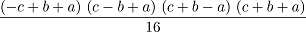
\includegraphics[keepaspectratio]{images/EMT4Geometry - Naila Khalidatus Salwa-134.png}}

\section{Aturan Triple Spread}\label{aturan-triple-spread}

Kerugian dari spread adalah bahwa mereka tidak lagi hanya menambahkan seperti sudut. Namun, tiga spread dari sebuah segitiga memenuhi aturan ``triple spread'' berikut ini.

\textgreater\&remvalue(sa,sb,sc); \$triplespread(sa,sb,sc)

\[\left({\it sc}+{\it sb}+{\it sa}\right)^2=2\,\left({\it sc}^2+  {\it sb}^2+{\it sa}^2\right)+4\,{\it sa}\,{\it sb}\,{\it sc}\]Aturan ini berlaku untuk tiga sudut yang berjumlah 180°.

\[\alpha+\beta+\gamma=\pi\]Karena spread dari

\[\alpha, \pi-\alpha\]sama, aturan triple spread juga benar, jika

\[\alpha+\beta=\gamma\]Karena penyebaran sudut negatif adalah sama, aturan penyebaran tiga kali lipat juga berlaku, jika

\[\alpha+\beta+\gamma=0\]Contohnya, kita bisa menghitung penyebaran sudut 60°. Ini adalah 3/4. Namun, persamaan ini memiliki solusi kedua, di mana semua penyebarannya adalah 0.

\textgreater\$solve(triplespread(x,x,x),x)

\[\left[ x=\frac{3}{4} , x=0 \right] \]Penyebaran 90° jelas adalah 1. Jika dua sudut ditambahkan ke 90°, penyebarannya menyelesaikan persamaan penyebaran tiga dengan a,b,1. Dengan perhitungan berikut, kita mendapatkan a + b = 1.

\textgreater\$triplespread(x,y,1), \$solve(\%,x)

\[\left[ x=1-y \right] \]\pandocbounded{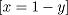
\includegraphics[keepaspectratio]{images/EMT4Geometry - Naila Khalidatus Salwa-142.png}}

Karena penyebaran 180°-t sama dengan penyebaran t, rumus penyebaran tiga kali lipat juga berlaku, jika satu sudut adalah jumlah atau selisih dari dua sudut lainnya.

Jadi kita dapat menemukan penyebaran sudut dua kali lipat. Perhatikan bahwa ada dua solusi lagi. Kita jadikan ini sebuah fungsi.

\textgreater\$solve(triplespread(a,a,x),x), function doublespread(a) \&= factor(rhs(\%{[}1{]}))

\[\left[ x=4\,a-4\,a^2 , x=0 \right] \]\\
- 4 (a - 1) a

\section{Sudut Pembagi}\label{sudut-pembagi}

Ini adalah situasi yang sudah kita ketahui.

\textgreater C\&:={[}0,0{]}; A\&:={[}4,0{]}; B\&:={[}0,3{]}; \ldots{}\\
\textgreater{} setPlotRange(-1,5,-1,5); \ldots{}\\
\textgreater{} plotPoint(A,``A''); plotPoint(B,``B''); plotPoint(C,``C''); \ldots{}\\
\textgreater{} plotSegment(B,A,``c''); plotSegment(A,C,``b''); plotSegment(C,B,``a''); \ldots{}\\
\textgreater{} insimg;

\begin{figure}
\centering
\pandocbounded{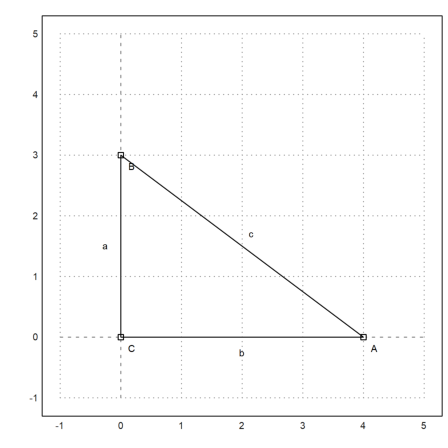
\includegraphics[keepaspectratio]{images/EMT4Geometry - Naila Khalidatus Salwa-144.png}}
\caption{images/EMT4Geometry\%20-\%20Naila\%20Khalidatus\%20Salwa-144.png}
\end{figure}

Mari kita hitung panjang garis bagi sudut di A. Tetapi kita ingin menyelesaikannya untuk a, b, c secara umum.

\textgreater\&remvalue(a,b,c);

Jadi, pertama-tama kita menghitung penyebaran sudut yang dibelah dua di A, menggunakan rumus penyebaran tiga.

Masalah dengan rumus ini muncul lagi. Rumus ini memiliki dua solusi. Kita harus memilih yang benar. Solusi lainnya mengacu pada sudut terbagi dua 180°-wa.

\textgreater\$triplespread(x,x,a/(a+b)), \$solve(\%,x), sa2 \&= rhs(\%{[}1{]}); \$sa2

\[\frac{-\sqrt{b^2+a\,b}+b+a}{2\,b+2\,a}\]\pandocbounded{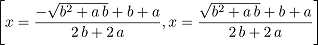
\includegraphics[keepaspectratio]{images/EMT4Geometry - Naila Khalidatus Salwa-146.png}}

\begin{figure}
\centering
\pandocbounded{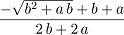
\includegraphics[keepaspectratio]{images/EMT4Geometry - Naila Khalidatus Salwa-147.png}}
\caption{images/EMT4Geometry\%20-\%20Naila\%20Khalidatus\%20Salwa-147.png}
\end{figure}

Mari kita periksa persegi panjang Egyptian.

\textgreater\$sa2 with {[}a=3\textsuperscript{2,b=4}2{]}

\[\frac{1}{10}\]Kita bisa mencetak sudut dalam Euler, setelah mentransfer penyebaran ke radian.

\textgreater wa2 := arcsin(sqrt(1/10)); degprint(wa2)

\begin{verbatim}
18°26'5.82''
\end{verbatim}

Titik P adalah perpotongan garis bagi sudut dengan sumbu y.

\textgreater P := {[}0,tan(wa2)*4{]}

\begin{verbatim}
[0,  1.33333]
\end{verbatim}

\textgreater plotPoint(P,``P''); plotSegment(A,P):

\begin{figure}
\centering
\pandocbounded{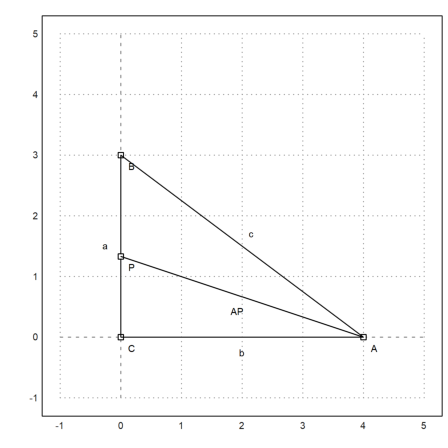
\includegraphics[keepaspectratio]{images/EMT4Geometry - Naila Khalidatus Salwa-149.png}}
\caption{images/EMT4Geometry\%20-\%20Naila\%20Khalidatus\%20Salwa-149.png}
\end{figure}

Mari kita periksa sudut-sudutnya dalam contoh spesifik kita.

\textgreater computeAngle(C,A,P), computeAngle(P,A,B)

\begin{verbatim}
0.321750554397
0.321750554397
\end{verbatim}

Sekarang kita hitung panjang garis bagi AP.

Kita menggunakan teorema sinus dalam segitiga APC. Teorema ini menyatakan bahwa

\[\frac{BC}{\sin(w_a)} = \frac{AC}{\sin(w_b)} = \frac{AB}{\sin(w_c)}\]memegang dalam segitiga apa pun. Kuadratkan, ini diterjemahkan ke dalam apa yang disebut ``hukum penyebaran''

\[\frac{a}{s_a} = \frac{b}{s_b} = \frac{c}{s_b}\]di mana a, b, c menunjukkan qudrah.

Karena spread CPA adalah 1-sa2, kita mendapatkan bisa/1=b/(1-sa2) dan bisa menghitung bisa (kuadran dari pembagi sudut).

\textgreater\&factor(ratsimp(b/(1-sa2))); bisa \&= \%; \$bisa

\[\frac{2\,b\,\left(b+a\right)}{\sqrt{b\,\left(b+a\right)}+b+a}\]Mari kita periksa rumus ini untuk nilai-nilai Egyptian kita.

\textgreater sqrt(mxmeval(``at(bisa,{[}a=3\textsuperscript{2,b=4}2{]})'')), distance(A,P)

\begin{verbatim}
4.21637021356
4.21637021356
\end{verbatim}

Kita juga dapat menghitung P menggunakan rumus penyebaran.

\textgreater py\&=factor(ratsimp(sa2*bisa)); \$py

\[-\frac{b\,\left(\sqrt{b\,\left(b+a\right)}-b-a\right)}{\sqrt{b\,  \left(b+a\right)}+b+a}\]Nilainya sama dengan yang kita dapatkan dengan rumus trigonometri.

\textgreater sqrt(mxmeval(``at(py,{[}a=3\textsuperscript{2,b=4}2{]})''))

\begin{verbatim}
1.33333333333
\end{verbatim}

\section{Sudut Akor}\label{sudut-akor}

Lihatlah situasi berikut ini.

\textgreater setPlotRange(1.2); \ldots{}\\
\textgreater{} color(1); plotCircle(circleWithCenter({[}0,0{]},1)); \ldots{}\\
\textgreater{} A:={[}cos(1),sin(1){]}; B:={[}cos(2),sin(2){]}; C:={[}cos(6),sin(6){]}; \ldots{}\\
\textgreater{} plotPoint(A,``A''); plotPoint(B,``B''); plotPoint(C,``C''); \ldots{}\\
\textgreater{} color(3); plotSegment(A,B,``c''); plotSegment(A,C,``b''); plotSegment(C,B,``a''); \ldots{}\\
\textgreater{} color(1); O:={[}0,0{]}; plotPoint(O,``0''); \ldots{}\\
\textgreater{} plotSegment(A,O); plotSegment(B,O); plotSegment(C,O,``r''); \ldots{}\\
\textgreater{} insimg;

\begin{figure}
\centering
\pandocbounded{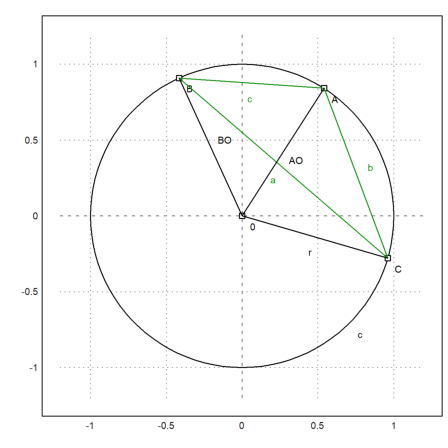
\includegraphics[keepaspectratio]{images/EMT4Geometry - Naila Khalidatus Salwa-154.png}}
\caption{images/EMT4Geometry\%20-\%20Naila\%20Khalidatus\%20Salwa-154.png}
\end{figure}

Kita dapat menggunakan Maxima untuk menyelesaikan rumus penyebaran tiga kali lipat untuk sudut-sudut di pusat O untuk r. Dengan demikian kita mendapatkan rumus untuk jari-jari kuadrat dari pericircle dalam hal kuadran sisi-sisinya.

Kali ini, Maxima menghasilkan beberapa angka nol yang rumit, yang kita abaikan.

\textgreater\&remvalue(a,b,c,r); // hapus nilai-nilai sebelumnya untuk perhitungan baru

\textgreater rabc \&= rhs(solve(triplespread(spread(b,r,r),spread(a,r,r),spread(c,r,r)),r){[}4{]}); \$rabc

\[-\frac{a\,b\,c}{c^2-2\,b\,c+a\,\left(-2\,c-2\,b\right)+b^2+a^2}\]Kita dapat menjadikannya sebuah fungsi Euler.

\textgreater function periradius(a,b,c) \&= rabc;

Mari kita periksa hasilnya untuk titik A, B, C.

\textgreater a:=quadrance(B,C); b:=quadrance(A,C); c:=quadrance(A,B);

Radiusnya memang 1.

\textgreater periradius(a,b,c)

\begin{verbatim}
1
\end{verbatim}

Faktanya adalah, bahwa penyebaran CBA hanya bergantung pada b dan c. Ini adalah teorema sudut akor.

\textgreater\$spread(b,a,c)*rabc \textbar{} ratsimp

\[\frac{b}{4}\]Pada kenyataannya, penyebarannya adalah b/(4r), dan kita melihat bahwa sudut chord b adalah setengah dari sudut tengah.

\textgreater\$doublespread(b/(4*r))-spread(b,r,r) \textbar{} ratsimp

\[0\]\# Contoh 6: Jarak Minimal pada Bidang

\section{Komentar awal}\label{komentar-awal}

Fungsi pada titik M di bidang, menetapkan jarak AM antara titik tetap A dan M, memiliki garis-garis level yang agak sederhana: lingkaran yang berpusat di A.

\textgreater\&remvalue();

\textgreater A={[}-1,-1{]};

\textgreater function d1(x,y):=sqrt((x-A{[}1{]})\textsuperscript{2+(y-A{[}2{]})}2)

\textgreater fcontour(``d1'',xmin=-2,xmax=0,ymin=-2,ymax=0,hue=1, \ldots{}\\
\textgreater{} title=``If you see ellipses, please set your window square''):

\begin{figure}
\centering
\pandocbounded{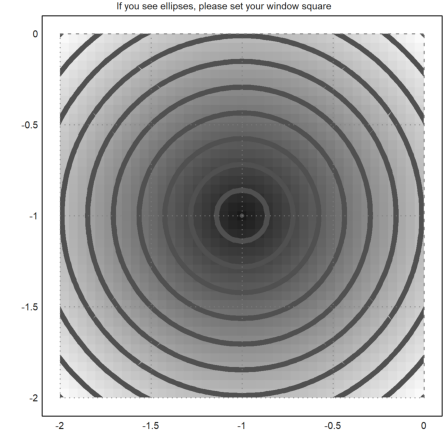
\includegraphics[keepaspectratio]{images/EMT4Geometry - Naila Khalidatus Salwa-158.png}}
\caption{images/EMT4Geometry\%20-\%20Naila\%20Khalidatus\%20Salwa-158.png}
\end{figure}

dan grafiknya juga cukup sederhana: bagian atas kerucut:

\textgreater plot3d(``d1'',xmin=-2,xmax=0,ymin=-2,ymax=0):

\begin{figure}
\centering
\pandocbounded{\includegraphics[keepaspectratio]{images/EMT4Geometry - Naila Khalidatus Salwa-159.png}}
\caption{images/EMT4Geometry\%20-\%20Naila\%20Khalidatus\%20Salwa-159.png}
\end{figure}

Tentu saja nilai minimum 0 dicapai di A.

\section{Dua titik}\label{dua-titik}

Sekarang kita lihat fungsi MA+MB di mana A dan B adalah dua titik (tetap). Ini adalah ``fakta yang terkenal'' bahwa kurva tingkat adalah elips, titik fokusnya adalah A dan B; kecuali AB minimum yang konstan pada segmen {[}AB{]}:

\textgreater B={[}1,-1{]};

\textgreater function d2(x,y):=d1(x,y)+sqrt((x-B{[}1{]})\textsuperscript{2+(y-B{[}2{]})}2)

\textgreater fcontour(``d2'',xmin=-2,xmax=2,ymin=-3,ymax=1,hue=1):

\begin{figure}
\centering
\pandocbounded{\includegraphics[keepaspectratio]{images/EMT4Geometry - Naila Khalidatus Salwa-160.png}}
\caption{images/EMT4Geometry\%20-\%20Naila\%20Khalidatus\%20Salwa-160.png}
\end{figure}

Grafiknya lebih menarik:

\textgreater plot3d(``d2'',xmin=-2,xmax=2,ymin=-3,ymax=1):

\begin{figure}
\centering
\pandocbounded{\includegraphics[keepaspectratio]{images/EMT4Geometry - Naila Khalidatus Salwa-161.png}}
\caption{images/EMT4Geometry\%20-\%20Naila\%20Khalidatus\%20Salwa-161.png}
\end{figure}

Pembatasan pada garis (AB) lebih terkenal:

\textgreater plot2d(``abs(x+1)+abs(x-1)'',xmin=-3,xmax=3):

\begin{figure}
\centering
\pandocbounded{\includegraphics[keepaspectratio]{images/EMT4Geometry - Naila Khalidatus Salwa-162.png}}
\caption{images/EMT4Geometry\%20-\%20Naila\%20Khalidatus\%20Salwa-162.png}
\end{figure}

\section{Tiga titik}\label{tiga-titik}

Sekarang, hal-hal menjadi tidak terlalu sederhana: Hal ini sedikit kurang dikenal bahwa MA+MB+MC mencapai minimum pada satu titik bidang, tetapi untuk menentukannya kurang sederhana:

\begin{enumerate}
\def\labelenumi{\arabic{enumi})}
\tightlist
\item
  Jika salah satu sudut segitiga ABC lebih dari 120° (katakanlah di A), maka minimum dicapai pada titik ini (katakanlah AB+AC).
\end{enumerate}

Contoh:

\textgreater C={[}-4,1{]};

\textgreater function d3(x,y):=d2(x,y)+sqrt((x-C{[}1{]})\textsuperscript{2+(y-C{[}2{]})}2)

\textgreater plot3d(``d3'',xmin=-5,xmax=3,ymin=-4,ymax=4);

\textgreater insimg;

\begin{figure}
\centering
\pandocbounded{\includegraphics[keepaspectratio]{images/EMT4Geometry - Naila Khalidatus Salwa-163.png}}
\caption{images/EMT4Geometry\%20-\%20Naila\%20Khalidatus\%20Salwa-163.png}
\end{figure}

\textgreater fcontour(``d3'',xmin=-4,xmax=1,ymin=-2,ymax=2,hue=1,title=``The minimum is on A'');

\textgreater P=(A\_B\_C\_A)'; plot2d(P{[}1{]},P{[}2{]},add=1,color=12);

\textgreater insimg;

\begin{figure}
\centering
\pandocbounded{\includegraphics[keepaspectratio]{images/EMT4Geometry - Naila Khalidatus Salwa-164.png}}
\caption{images/EMT4Geometry\%20-\%20Naila\%20Khalidatus\%20Salwa-164.png}
\end{figure}

\begin{enumerate}
\def\labelenumi{\arabic{enumi})}
\setcounter{enumi}{1}
\tightlist
\item
  Tetapi jika semua sudut segitiga ABC kurang dari 120°, minimumnya adalah pada titik F di bagian dalam segitiga, yang merupakan satu-satunya titik yang melihat sisi-sisi ABC dengan sudut yang sama (masing-masing 120°):
\end{enumerate}

\textgreater C={[}-0.5,1{]};

\textgreater plot3d(``d3'',xmin=-2,xmax=2,ymin=-2,ymax=2):

\begin{figure}
\centering
\pandocbounded{\includegraphics[keepaspectratio]{images/EMT4Geometry - Naila Khalidatus Salwa-165.png}}
\caption{images/EMT4Geometry\%20-\%20Naila\%20Khalidatus\%20Salwa-165.png}
\end{figure}

\textgreater fcontour(``d3'',xmin=-2,xmax=2,ymin=-2,ymax=2,hue=1,title=``The Fermat point'');

\textgreater P=(A\_B\_C\_A)'; plot2d(P{[}1{]},P{[}2{]},add=1,color=12);

\textgreater insimg;

\begin{figure}
\centering
\pandocbounded{\includegraphics[keepaspectratio]{images/EMT4Geometry - Naila Khalidatus Salwa-166.png}}
\caption{images/EMT4Geometry\%20-\%20Naila\%20Khalidatus\%20Salwa-166.png}
\end{figure}

Merupakan kegiatan yang menarik untuk merealisasikan gambar di atas dengan perangkat lunak geometri; sebagai contoh, saya tahu sebuah perangkat lunak yang ditulis dalam bahasa Java yang memiliki instruksi ``garis kontur''\ldots{}

Semua hal di atas telah ditemukan oleh seorang hakim Perancis bernama Pierre de Fermat; dia menulis surat kepada para ahli lain seperti pendeta Marin Mersenne dan Blaise Pascal yang bekerja di bagian pajak penghasilan. Jadi titik unik F sedemikian rupa sehingga FA+FB+FC minimal, disebut titik Fermat dari segitiga. Namun tampaknya beberapa tahun sebelumnya, Torriccelli dari Italia telah menemukan titik ini sebelum Fermat menemukannya! Tradisi yang berlaku adalah mencatat titik F ini\ldots{}

\section{Optmasi Titik pada Empat titik}\label{optmasi-titik-pada-empat-titik}

Langkah selanjutnya adalah menambahkan titik ke-4 D dan mencoba meminimalkan MA+MB+MC+MD; misalkan Anda adalah operator TV kabel dan ingin menemukan di bidang mana Anda harus meletakkan antena Anda sehingga Anda dapat memberi makan empat desa dan menggunakan panjang kabel sesedikit mungkin!

\textgreater D={[}1,1{]};

\textgreater function d4(x,y):=d3(x,y)+sqrt((x-D{[}1{]})\textsuperscript{2+(y-D{[}2{]})}2)

\textgreater plot3d(``d4'',xmin=-1.5,xmax=1.5,ymin=-1.5,ymax=1.5):

\begin{figure}
\centering
\pandocbounded{\includegraphics[keepaspectratio]{images/EMT4Geometry - Naila Khalidatus Salwa-167.png}}
\caption{images/EMT4Geometry\%20-\%20Naila\%20Khalidatus\%20Salwa-167.png}
\end{figure}

\textgreater fcontour(``d4'',xmin=-1.5,xmax=1.5,ymin=-1.5,ymax=1.5,hue=1);

\textgreater P=(A\_B\_C\_D)'; plot2d(P{[}1{]},P{[}2{]},points=1,add=1,color=12);

\textgreater insimg;

\begin{figure}
\centering
\pandocbounded{\includegraphics[keepaspectratio]{images/EMT4Geometry - Naila Khalidatus Salwa-168.png}}
\caption{images/EMT4Geometry\%20-\%20Naila\%20Khalidatus\%20Salwa-168.png}
\end{figure}

Masih ada nilai minimum dan tidak ada simpul A, B, C atau D yang tercapai:

\textgreater function f(x):=d4(x{[}1{]},x{[}2{]})

\textgreater neldermin(``f'',{[}0.2,0.2{]})

\begin{verbatim}
[0,  0]
\end{verbatim}

Tampaknya dalam kasus ini, koordinat titik optimal adalah rasional atau mendekati rasional\ldots{}

Karena ABCD adalah sebuah bujur sangkar, maka kita berharap bahwa titik optimalnya adalah pusat dari ABCD:

\textgreater C={[}-1,1{]};

\textgreater plot3d(``d4'',xmin=-1,xmax=1,ymin=-1,ymax=1):

\begin{figure}
\centering
\pandocbounded{\includegraphics[keepaspectratio]{images/EMT4Geometry - Naila Khalidatus Salwa-169.png}}
\caption{images/EMT4Geometry\%20-\%20Naila\%20Khalidatus\%20Salwa-169.png}
\end{figure}

\textgreater fcontour(``d4'',xmin=-1.5,xmax=1.5,ymin=-1.5,ymax=1.5,hue=1);

\textgreater P=(A\_B\_C\_D)'; plot2d(P{[}1{]},P{[}2{]},add=1,color=12,points=1);

\textgreater insimg;

\begin{figure}
\centering
\pandocbounded{\includegraphics[keepaspectratio]{images/EMT4Geometry - Naila Khalidatus Salwa-170.png}}
\caption{images/EMT4Geometry\%20-\%20Naila\%20Khalidatus\%20Salwa-170.png}
\end{figure}

\chapter{Contoh 7: Bola Dandelin dengan Povray}\label{contoh-7-bola-dandelin-dengan-povray}

Anda dapat menjalankan demonstrasi ini, jika Anda telah menginstal Povray, dan pvengine.exe pada jalur program.

Pertama, kita menghitung jari-jari bola.

Jika Anda melihat gambar di bawah ini, Anda dapat melihat bahwa kita membutuhkan dua buah lingkaran yang bersinggungan dengan dua buah garis yang membentuk kerucut, dan satu buah garis yang membentuk bidang yang memotong kerucut.

Kita menggunakan file geometri.e dari Euler untuk hal ini.

\textgreater load geometry;

Pertama, dua garis yang membentuk kerucut.

\textgreater g1 \&= lineThrough({[}0,0{]},{[}1,a{]})

\begin{verbatim}
                             [- a, 1, 0]
\end{verbatim}

\textgreater g2 \&= lineThrough({[}0,0{]},{[}-1,a{]})

\begin{verbatim}
                            [- a, - 1, 0]
\end{verbatim}

Kemudian baris ketiga.

\textgreater g \&= lineThrough({[}-1,0{]},{[}1,1{]})

\begin{verbatim}
                             [- 1, 2, 1]
\end{verbatim}

Kami merencanakan semuanya sejauh ini.

\textgreater setPlotRange(-1,1,0,2);

\textgreater color(black); plotLine(g(),``\,``)

\textgreater a:=2; color(blue); plotLine(g1(),``\,``), plotLine(g2(),''\,``):

\begin{figure}
\centering
\pandocbounded{\includegraphics[keepaspectratio]{images/EMT4Geometry - Naila Khalidatus Salwa-171.png}}
\caption{images/EMT4Geometry\%20-\%20Naila\%20Khalidatus\%20Salwa-171.png}
\end{figure}

Sekarang, kita ambil titik umum pada sumbu y.

\textgreater P \&= {[}0,u{]}

\begin{verbatim}
                                [0, u]
\end{verbatim}

Hitung jarak ke g1.

\textgreater d1 \&= distance(P,projectToLine(P,g1)); \$d1

\[\sqrt{\left(\frac{a^2\,u}{a^2+1}-u\right)^2+\frac{a^2\,u^2}{\left(a  ^2+1\right)^2}}\]Hitung jarak ke g.

\textgreater d \&= distance(P,projectToLine(P,g)); \$d

\[\sqrt{\left(\frac{u+2}{5}-u\right)^2+\frac{\left(2\,u-1\right)^2}{  25}}\]Dan temukan pusat kedua lingkaran, yang jaraknya sama.

\textgreater sol \&= solve(d1\textsuperscript{2=d}2,u); \$sol

\[\left[ u=\frac{-\sqrt{5}\,\sqrt{a^2+1}+2\,a^2+2}{4\,a^2-1} , u=  \frac{\sqrt{5}\,\sqrt{a^2+1}+2\,a^2+2}{4\,a^2-1} \right] \]Ada dua solusi.

Kami mengevaluasi solusi simbolis, dan menemukan kedua pusat, dan kedua jarak.

\textgreater u := sol()

\begin{verbatim}
[0.333333,  1]
\end{verbatim}

\textgreater dd := d()

\begin{verbatim}
[0.149071,  0.447214]
\end{verbatim}

Plot lingkaran ke dalam gambar.

\textgreater color(red);

\textgreater plotCircle(circleWithCenter({[}0,u{[}1{]}{]},dd{[}1{]}),``\,``);

\textgreater plotCircle(circleWithCenter({[}0,u{[}2{]}{]},dd{[}2{]}),``\,``);

\textgreater insimg;

\begin{figure}
\centering
\pandocbounded{\includegraphics[keepaspectratio]{images/EMT4Geometry - Naila Khalidatus Salwa-175.png}}
\caption{images/EMT4Geometry\%20-\%20Naila\%20Khalidatus\%20Salwa-175.png}
\end{figure}

\section{Plot dengan Povray}\label{plot-dengan-povray}

Selanjutnya kita plot semuanya dengan Povray. Perhatikan bahwa Anda mengubah perintah apa pun dalam urutan perintah Povray berikut ini, dan jalankan kembali semua perintah dengan Shift-Return.

Pertama kita memuat fungsi povray.

\textgreater load povray;

\textgreater defaultpovray=``C:\textbackslash Program Files\textbackslash POV-Ray\textbackslash v3.7\textbackslash bin\textbackslash pvengine.exe''

\begin{verbatim}
C:\Program Files\POV-Ray\v3.7\bin\pvengine.exe
\end{verbatim}

Kami menyiapkan pemandangan dengan tepat.

\textgreater povstart(zoom=11,center={[}0,0,0.5{]},height=10°,angle=140°);

Selanjutnya kita menulis dua bola ke file Povray.

\textgreater writeln(povsphere({[}0,0,u{[}1{]}{]},dd{[}1{]},povlook(red)));

\textgreater writeln(povsphere({[}0,0,u{[}2{]}{]},dd{[}2{]},povlook(red)));

Dan kerucutnya, transparan.

\textgreater writeln(povcone({[}0,0,0{]},0,{[}0,0,a{]},1,povlook(lightgray,1)));

Kami menghasilkan bidang yang terbatas pada kerucut.

\textgreater gp=g();

\textgreater pc=povcone({[}0,0,0{]},0,{[}0,0,a{]},1,``\,``);

\textgreater vp={[}gp{[}1{]},0,gp{[}2{]}{]}; dp=gp{[}3{]};

\textgreater writeln(povplane(vp,dp,povlook(blue,0.5),pc));

Sekarang kita menghasilkan dua titik pada lingkaran, di mana bola menyentuh kerucut.

\textgreater function turnz(v) := return

\textgreater P1=projectToLine({[}0,u{[}1{]}{]},g1()); P1=turnz({[}P1{[}1{]},0,P1{[}2{]}{]});

\textgreater writeln(povpoint(P1,povlook(yellow)));

\textgreater P2=projectToLine({[}0,u{[}2{]}{]},g1()); P2=turnz({[}P2{[}1{]},0,P2{[}2{]}{]});

\textgreater writeln(povpoint(P2,povlook(yellow)));

Kemudian kami menghasilkan dua titik di mana bola menyentuh bidang. Ini adalah fokus elips.

\textgreater P3=projectToLine({[}0,u{[}1{]}{]},g()); P3={[}P3{[}1{]},0,P3{[}2{]}{]};

\textgreater writeln(povpoint(P3,povlook(yellow)));

\textgreater P4=projectToLine({[}0,u{[}2{]}{]},g()); P4={[}P4{[}1{]},0,P4{[}2{]}{]};

\textgreater writeln(povpoint(P4,povlook(yellow)));

Selanjutnya kita menghitung perpotongan P1P2 dengan bidang.

\textgreater t1=scalp(vp,P1)-dp; t2=scalp(vp,P2)-dp; P5=P1+t1/(t1-t2)*(P2-P1);

\textgreater writeln(povpoint(P5,povlook(yellow)));

Kami menghubungkan titik-titik dengan segmen garis.

\textgreater writeln(povsegment(P1,P2,povlook(yellow)));

\textgreater writeln(povsegment(P5,P3,povlook(yellow)));

\textgreater writeln(povsegment(P5,P4,povlook(yellow)));

Sekarang, kita menghasilkan pita abu-abu, di mana bola-bola menyentuh kerucut.

\textgreater pcw=povcone({[}0,0,0{]},0,{[}0,0,a{]},1.01);

\textgreater pc1=povcylinder({[}0,0,P1{[}3{]}-defaultpointsize/2{]},{[}0,0,P1{[}3{]}+defaultpointsize/2{]},1);

\textgreater writeln(povintersection({[}pcw,pc1{]},povlook(gray)));

\textgreater pc2=povcylinder({[}0,0,P2{[}3{]}-defaultpointsize/2{]},{[}0,0,P2{[}3{]}+defaultpointsize/2{]},1);

\textgreater writeln(povintersection({[}pcw,pc2{]},povlook(gray)));

Mulai program Povray.

\textgreater povend();

\begin{figure}
\centering
\pandocbounded{\includegraphics[keepaspectratio]{images/EMT4Geometry - Naila Khalidatus Salwa-176.png}}
\caption{images/EMT4Geometry\%20-\%20Naila\%20Khalidatus\%20Salwa-176.png}
\end{figure}

Untuk mendapatkan Anaglyph ini, kita perlu menempatkan semuanya ke dalam fungsi scene. Fungsi ini akan digunakan dua kali nanti.

\textgreater function scene () \ldots{}

\begin{verbatim}
global a,u,dd,g,g1,defaultpointsize;
writeln(povsphere([0,0,u[1]],dd[1],povlook(red)));
writeln(povsphere([0,0,u[2]],dd[2],povlook(red)));
writeln(povcone([0,0,0],0,[0,0,a],1,povlook(lightgray,1)));
gp=g();
pc=povcone([0,0,0],0,[0,0,a],1,"");
vp=[gp[1],0,gp[2]]; dp=gp[3];
writeln(povplane(vp,dp,povlook(blue,0.5),pc));
P1=projectToLine([0,u[1]],g1()); P1=turnz([P1[1],0,P1[2]]);
writeln(povpoint(P1,povlook(yellow)));
P2=projectToLine([0,u[2]],g1()); P2=turnz([P2[1],0,P2[2]]);
writeln(povpoint(P2,povlook(yellow)));
P3=projectToLine([0,u[1]],g()); P3=[P3[1],0,P3[2]];
writeln(povpoint(P3,povlook(yellow)));
P4=projectToLine([0,u[2]],g()); P4=[P4[1],0,P4[2]];
writeln(povpoint(P4,povlook(yellow)));
t1=scalp(vp,P1)-dp; t2=scalp(vp,P2)-dp; P5=P1+t1/(t1-t2)*(P2-P1);
writeln(povpoint(P5,povlook(yellow)));
writeln(povsegment(P1,P2,povlook(yellow)));
writeln(povsegment(P5,P3,povlook(yellow)));
writeln(povsegment(P5,P4,povlook(yellow)));
pcw=povcone([0,0,0],0,[0,0,a],1.01);
pc1=povcylinder([0,0,P1[3]-defaultpointsize/2],[0,0,P1[3]+defaultpointsize/2],1);
writeln(povintersection([pcw,pc1],povlook(gray)));
pc2=povcylinder([0,0,P2[3]-defaultpointsize/2],[0,0,P2[3]+defaultpointsize/2],1);
writeln(povintersection([pcw,pc2],povlook(gray)));
endfunction
\end{verbatim}

Anda memerlukan kacamata merah/sian untuk mengapresiasi efek berikut ini.

\textgreater povanaglyph(``scene'',zoom=11,center={[}0,0,0.5{]},height=10°,angle=140°);

\begin{figure}
\centering
\pandocbounded{\includegraphics[keepaspectratio]{images/EMT4Geometry - Naila Khalidatus Salwa-177.png}}
\caption{images/EMT4Geometry\%20-\%20Naila\%20Khalidatus\%20Salwa-177.png}
\end{figure}

\chapter{Contoh 8: Geometri Bumi}\label{contoh-8-geometri-bumi}

Pada buku catatan ini, kita ingin melakukan beberapa komputasi bola. Fungsi-fungsi tersebut terdapat pada file ``spherical.e'' pada folder contoh. Kita perlu memuat file tersebut terlebih dahulu.

\textgreater load ``spherical.e'';

Untuk memasukkan posisi geografis, kami menggunakan vektor dengan dua koordinat dalam radian (utara dan timur, nilai negatif untuk selatan dan barat). Berikut ini adalah koordinat untuk Kampus FMIPA UNY.

\textgreater FMIPA={[}rad(-7,-46.467),rad(110,23.05){]}

\begin{verbatim}
[-0.13569,  1.92657]
\end{verbatim}

Anda dapat mencetak posisi ini dengan sposprint (cetak posisi bola).

\textgreater sposprint(FMIPA) // posisi garis lintang dan garis bujur FMIPA UNY

\begin{verbatim}
S 7°46.467' E 110°23.050'
\end{verbatim}

Mari kita tambahkan dua kota lagi, Solo dan Semarang.

\textgreater Solo={[}rad(-7,-34.333),rad(110,49.683){]}; Semarang={[}rad(-6,-59.05),rad(110,24.533){]};

\textgreater sposprint(Solo), sposprint(Semarang),

\begin{verbatim}
S 7°34.333' E 110°49.683'
S 6°59.050' E 110°24.533'
\end{verbatim}

Pertama, kita menghitung vektor dari satu titik ke titik lainnya pada bola ideal. Vektor ini adalah {[}heading, jarak{]} dalam radian. Untuk menghitung jarak di bumi, kita kalikan dengan jari-jari bumi pada garis lintang 7°.

\textgreater br=svector(FMIPA,Solo); degprint(br{[}1{]}), br{[}2{]}*rearth(7°)-\textgreater km // perkiraan jarak FMIPA-Solo

\begin{verbatim}
65°20'26.60''
53.8945384608
\end{verbatim}

Ini adalah perkiraan yang baik. Rutinitas berikut ini menggunakan perkiraan yang lebih baik lagi. Pada jarak yang pendek, hasilnya hampir sama.

\textgreater esdist(FMIPA,Semarang)-\textgreater'' km'', // perkiraan jarak FMIPA-Semarang

\begin{verbatim}
88.0114026318 km
\end{verbatim}

Ada fungsi untuk pos, dengan mempertimbangkan bentuk bumi yang elips. Sekali lagi, kami mencetak dengan cara yang canggih.

\textgreater sdegprint(esdir(FMIPA,Solo))

\begin{verbatim}
     65.34°
\end{verbatim}

Sudut segitiga melebihi 180° pada bola.

\textgreater asum=sangle(Solo,FMIPA,Semarang)+sangle(FMIPA,Solo,Semarang)+sangle(FMIPA,Semarang,Solo); degprint(asum)

\begin{verbatim}
180°0'10.77''
\end{verbatim}

Ini dapat digunakan untuk menghitung luas segitiga. Catatan: Untuk segitiga kecil, cara ini tidak akurat karena kesalahan pengurangan dalam asum-pi.

\textgreater(asum-pi)*rearth(48°)\^{}2-\textgreater'' km\^{}2'', // perkiraan luas segitiga FMIPA-Solo-Semarang

\begin{verbatim}
2116.02948749 km^2
\end{verbatim}

Ada sebuah fungsi untuk hal ini, yang menggunakan garis lintang rata-rata segitiga untuk menghitung radius bumi, dan menangani kesalahan pembulatan untuk segitiga yang sangat kecil.

\textgreater esarea(Solo,FMIPA,Semarang)-\textgreater'' km\^{}2'', //perkiraan yang sama dengan fungsi esarea()

\begin{verbatim}
2123.64310526 km^2
\end{verbatim}

Kita juga dapat menambahkan vektor ke posisi. Sebuah vektor berisi arah dan jarak, keduanya dalam radian. Untuk mendapatkan sebuah vektor, kita menggunakan svector. Untuk menambahkan sebuah vektor ke sebuah posisi, kita menggunakan saddvector.

\textgreater v=svector(FMIPA,Solo); sposprint(saddvector(FMIPA,v)), sposprint(Solo),

\begin{verbatim}
S 7°34.333' E 110°49.683'
S 7°34.333' E 110°49.683'
\end{verbatim}

Fungsi-fungsi ini mengasumsikan bola yang ideal. Hal yang sama di bumi.

\textgreater sposprint(esadd(FMIPA,esdir(FMIPA,Solo),esdist(FMIPA,Solo))), sposprint(Solo),

\begin{verbatim}
S 7°34.333' E 110°49.683'
S 7°34.333' E 110°49.683'
\end{verbatim}

Mari kita beralih ke contoh yang lebih besar, Tugu Jogja dan Monas Jakarta (menggunakan Google Earth untuk mencari koordinatnya).

\textgreater Tugu={[}-7.7833°,110.3661°{]}; Monas={[}-6.175°,106.811944°{]};

\textgreater sposprint(Tugu), sposprint(Monas)

\begin{verbatim}
S 7°46.998' E 110°21.966'
S 6°10.500' E 106°48.717'
\end{verbatim}

Menurut Google Earth, jaraknya adalah 429,66 km. Kami mendapatkan perkiraan yang bagus.

\textgreater esdist(Tugu,Monas)-\textgreater{} ``km'', // perkiraan jarak Tugu Jogja - Monas Jakarta

\begin{verbatim}
431.565659488km
\end{verbatim}

Judulnya sama dengan yang dihitung di Google Earth.

\textgreater degprint(esdir(Tugu,Monas))

\begin{verbatim}
294°17'2.85''
\end{verbatim}

Namun, kita tidak lagi mendapatkan posisi target yang tepat, jika kita menambahkan heading dan jarak ke posisi semula. Hal ini terjadi, karena kita tidak menghitung fungsi inversi secara tepat, tetapi mengambil perkiraan radius bumi di sepanjang jalur.

\textgreater sposprint(esadd(Tugu,esdir(Tugu,Monas),esdist(Tugu,Monas)))

\begin{verbatim}
S 6°10.500' E 106°48.717'
\end{verbatim}

Namun demikian, kesalahannya tidak besar.

\textgreater sposprint(Monas),

\begin{verbatim}
S 6°10.500' E 106°48.717'
\end{verbatim}

Tentu saja, kita tidak bisa berlayar dengan arah yang sama dari satu tujuan ke tujuan lainnya, jika kita ingin mengambil jalur terpendek. Bayangkan, Anda terbang ke arah NE mulai dari titik mana pun di bumi. Kemudian Anda akan berputar ke kutub utara. Lingkaran besar tidak mengikuti arah yang konstan!

Perhitungan berikut ini menunjukkan bahwa kita akan melenceng dari tujuan yang benar, jika kita menggunakan arah yang sama selama perjalanan.

\textgreater dist=esdist(Tugu,Monas); hd=esdir(Tugu,Monas);

Sekarang kita tambahkan 10 kali sepersepuluh dari jarak tersebut, dengan menggunakan arah ke Monas, kita sampai di Tugu.

\textgreater p=Tugu; loop 1 to 10; p=esadd(p,hd,dist/10); end;

Hasilnya berbeda jauh.

\textgreater sposprint(p), skmprint(esdist(p,Monas))

\begin{verbatim}
S 6°11.250' E 106°48.372'
     1.529km
\end{verbatim}

Sebagai contoh lain, mari kita ambil dua titik di bumi pada garis lintang yang sama.

\textgreater P1={[}30°,10°{]}; P2={[}30°,50°{]};

Jalur terpendek dari P1 ke P2 bukanlah lingkaran lintang 30°, tetapi jalur yang lebih pendek yang dimulai 10° lebih jauh ke utara di P1.

\textgreater sdegprint(esdir(P1,P2))

\begin{verbatim}
     79.69°
\end{verbatim}

Namun, jika kita mengikuti pembacaan kompas ini, kita akan berputar ke kutub utara! Jadi, kita harus menyesuaikan arah kita di sepanjang jalan. Untuk tujuan kasar, kita menyesuaikannya pada 1/10 dari jarak total.

\textgreater p=P1; dist=esdist(P1,P2); \ldots{}\\
\textgreater{} loop 1 to 10; dir=esdir(p,P2); sdegprint(dir), p=esadd(p,dir,dist/10); end;

\begin{verbatim}
     79.69°
     81.67°
     83.71°
     85.78°
     87.89°
     90.00°
     92.12°
     94.22°
     96.29°
     98.33°
\end{verbatim}

Jaraknya tidak tepat, karena kita akan menambahkan sedikit kesalahan, jika kita mengikuti judul yang sama terlalu lama.

\textgreater skmprint(esdist(p,P2))

\begin{verbatim}
     0.203km
\end{verbatim}

Kami mendapatkan perkiraan yang baik, jika kami menyesuaikan arah setiap 1/100 dari total jarak dari Tugu ke Monas.

\textgreater p=Tugu; dist=esdist(Tugu,Monas); \ldots{}\\
\textgreater{} loop 1 to 100; p=esadd(p,esdir(p,Monas),dist/100); end;

\textgreater skmprint(esdist(p,Monas))

\begin{verbatim}
     0.000km
\end{verbatim}

Untuk keperluan navigasi, kita bisa mendapatkan urutan posisi GPS di sepanjang Bundaran HI menuju Monas dengan fungsi navigate.

\textgreater load spherical; v=navigate(Tugu,Monas,10); \ldots{}\\
\textgreater{} loop 1 to rows(v); sposprint(v{[}\#{]}), end;

\begin{verbatim}
S 7°46.998' E 110°21.966'
S 7°37.422' E 110°0.573'
S 7°27.829' E 109°39.196'
S 7°18.219' E 109°17.834'
S 7°8.592' E 108°56.488'
S 6°58.948' E 108°35.157'
S 6°49.289' E 108°13.841'
S 6°39.614' E 107°52.539'
S 6°29.924' E 107°31.251'
S 6°20.219' E 107°9.977'
S 6°10.500' E 106°48.717'
\end{verbatim}

Kami menulis sebuah fungsi, yang memetakan bumi, dua posisi, dan posisi di antaranya.

\textgreater function testplot \ldots{}

\begin{verbatim}
useglobal;
plotearth;
plotpos(Tugu,"Tugu Jogja"); plotpos(Monas,"Tugu Monas");
plotposline(v);
endfunction
\end{verbatim}

Sekarang rencanakan semuanya.

\textgreater plot3d(``testplot'',angle=25, height=6,\textgreater own,\textgreater user,zoom=4):

\begin{figure}
\centering
\pandocbounded{\includegraphics[keepaspectratio]{images/EMT4Geometry - Naila Khalidatus Salwa-178.png}}
\caption{images/EMT4Geometry\%20-\%20Naila\%20Khalidatus\%20Salwa-178.png}
\end{figure}

Atau, gunakan plot3d untuk mendapatkan tampilan anaglyph-nya. Ini terlihat sangat bagus dengan kacamata merah/cyan.

\textgreater plot3d(``testplot'',angle=25,height=6,distance=5,own=1,anaglyph=1,zoom=4):

\begin{figure}
\centering
\pandocbounded{\includegraphics[keepaspectratio]{images/EMT4Geometry - Naila Khalidatus Salwa-179.png}}
\caption{images/EMT4Geometry\%20-\%20Naila\%20Khalidatus\%20Salwa-179.png}
\end{figure}

\chapter{Latihan}\label{latihan-1}

\begin{enumerate}
\def\labelenumi{\arabic{enumi}.}
\tightlist
\item
  Gambarlah segi-n beraturan jika diketahui titik pusat O, n, dan jarak titik pusat ke titik-titik sudut segi-n tersebut (jari-jari lingkaran luar segi-n), r.
\end{enumerate}

Petunjuk:

\begin{itemize}
\item
  Besar sudut pusat yang menghadap masing-masing sisi segi-n adalah
\item
  (360/n).
\item
  Titik-titik sudut segi-n merupakan perpotongan lingkaran luar segi-n
\item
  dan garis-garis yang melalui pusat dan saling membentuk sudut sebesar
\item
  kelipatan (360/n).
\item
  Untuk n ganjil, pilih salah satu titik sudut adalah di atas.
\item
  Untuk n genap, pilih 2 titik di kanan dan kiri lurus dengan titik
\item
  pusat.
\item
  Anda dapat menggambar segi-3, 4, 5, 6, 7, dst beraturan.
\end{itemize}

\textgreater load geometry

\begin{verbatim}
Numerical and symbolic geometry.
\end{verbatim}

\textgreater setPlotRange (-5,5,-5,5);

\textgreater A = {[}-3,-3{]}; plotPoint(A,``A''):

\begin{figure}
\centering
\pandocbounded{\includegraphics[keepaspectratio]{images/EMT4Geometry - Naila Khalidatus Salwa-180.png}}
\caption{images/EMT4Geometry\%20-\%20Naila\%20Khalidatus\%20Salwa-180.png}
\end{figure}

\textgreater B = {[}3, -3{]}; plotPoint(B,``B''):

\begin{figure}
\centering
\pandocbounded{\includegraphics[keepaspectratio]{images/EMT4Geometry - Naila Khalidatus Salwa-181.png}}
\caption{images/EMT4Geometry\%20-\%20Naila\%20Khalidatus\%20Salwa-181.png}
\end{figure}

\textgreater C = {[}0, 4{]} ; plotPoint(C,``C''):

\begin{figure}
\centering
\pandocbounded{\includegraphics[keepaspectratio]{images/EMT4Geometry - Naila Khalidatus Salwa-182.png}}
\caption{images/EMT4Geometry\%20-\%20Naila\%20Khalidatus\%20Salwa-182.png}
\end{figure}

\textgreater plotSegment(A, B,``c'');

\textgreater plotSegment(B, C, ``a'');

\textgreater plotSegment(A, C, ``b'');

\textgreater aspect(1):

\begin{figure}
\centering
\pandocbounded{\includegraphics[keepaspectratio]{images/EMT4Geometry - Naila Khalidatus Salwa-183.png}}
\caption{images/EMT4Geometry\%20-\%20Naila\%20Khalidatus\%20Salwa-183.png}
\end{figure}

\textgreater c=circleThrough(A,B,C);

\textgreater R=getCircleRadius(c);

\textgreater O=getCircleCenter(c);

\textgreater plotPoint(O,``O'');

\textgreater l=angleBisector(A,C,B);

\textgreater color(5); plotLine(l); color(1);

\textgreater plotCircle(c, ``Lingkaran luar Segitiga ABC''):

\begin{figure}
\centering
\pandocbounded{\includegraphics[keepaspectratio]{images/EMT4Geometry - Naila Khalidatus Salwa-184.png}}
\caption{images/EMT4Geometry\%20-\%20Naila\%20Khalidatus\%20Salwa-184.png}
\end{figure}

\begin{enumerate}
\def\labelenumi{\arabic{enumi}.}
\setcounter{enumi}{1}
\tightlist
\item
  Gambarlah suatu parabola yang melalui 3 titik yang diketahui.
\end{enumerate}

Petunjuk:

\begin{itemize}
\item
  Misalkan persamaan parabolanya y= ax\^{}2+bx+c.
\item
  Substitusikan koordinat titik-titik yang diketahui ke persamaan tersebut.
\item
  Selesaikan SPL yang terbentuk untuk mendapatkan nilai-nilai a, b, c.
\end{itemize}

\textgreater setPlotRange(5); D={[}-1,0{]}; E={[}-4,0{]}; F={[}0,-4{]};

\textgreater plotPoint(D,``D''); plotPoint(E, ``E''); plotPoint(F,``F''):

\begin{figure}
\centering
\pandocbounded{\includegraphics[keepaspectratio]{images/EMT4Geometry - Naila Khalidatus Salwa-185.png}}
\caption{images/EMT4Geometry\%20-\%20Naila\%20Khalidatus\%20Salwa-185.png}
\end{figure}

\textgreater sol \&= solve ({[}a+b=-c, 16*a+4*b=-c, c=-4{]}, {[}a, b, c{]})

\begin{verbatim}
                     [[a = - 1, b = 5, c = - 4]]
\end{verbatim}

\textgreater function y(x) \&= -x\^{}2-5*x-4

\begin{verbatim}
                               2
                            - x  - 5 x - 4
\end{verbatim}

\textgreater plot2d(``y'',-5,5,-5,5):

\begin{figure}
\centering
\pandocbounded{\includegraphics[keepaspectratio]{images/EMT4Geometry - Naila Khalidatus Salwa-186.png}}
\caption{images/EMT4Geometry\%20-\%20Naila\%20Khalidatus\%20Salwa-186.png}
\end{figure}

\begin{enumerate}
\def\labelenumi{\arabic{enumi}.}
\setcounter{enumi}{2}
\item
  Gambarlah suatu segi-4 yang diketahui keempat titik sudutnya, misalnya A, B, C, D.

  \begin{itemize}
  \item
    Tentukan apakah segi-4 tersebut merupakan segi-4 garis singgung (sisinya-sisintya merupakan garis singgung lingkaran yang sama yakni lingkaran dalam segi-4 tersebut).
  \item
    Suatu segi-4 merupakan segi-4 garis singgung apabila keempat garis bagi sudutnya bertemu di satu titik.
  \item
    Jika segi-4 tersebut merupakan segi-4 garis singgung, gambar lingkaran dalamnya.
  \item
    Tunjukkan bahwa syarat suatu segi-4 merupakan segi-4 garis singgung apabila hasil kali panjang sisi-sisi yang berhadapan sama.
  \end{itemize}
\end{enumerate}

\textgreater load geometry

\begin{verbatim}
Numerical and symbolic geometry.
\end{verbatim}

\textgreater setPlotRange(-5,5,-5,5);

\textgreater A={[}-4,-4{]}; plotPoint(A,``A'');\ldots{}\\
\textgreater{} B={[}4,-4{]}; plotPoint(B,``B'');\ldots{}\\
\textgreater{} C={[}4,4{]}; plotPoint(C,``C'');\ldots{}\\
\textgreater{} D={[}-4,4{]}; plotPoint(D,``D'');

\textgreater plotSegment(A,B,``\,``);\ldots{}\\
\textgreater{} plotSegment(B,C,''``);\ldots{}\\
\textgreater{} plotSegment(C,D,''``);\ldots{}\\
\textgreater{} plotSegment(A,D,''\,``);

\textgreater aspect(1):

\begin{figure}
\centering
\pandocbounded{\includegraphics[keepaspectratio]{images/EMT4Geometry - Naila Khalidatus Salwa-187.png}}
\caption{images/EMT4Geometry\%20-\%20Naila\%20Khalidatus\%20Salwa-187.png}
\end{figure}

\textgreater l=angleBisector(A,B,C); m=angleBisector(B,C,D);

\textgreater P=lineIntersection(l,m);

\textgreater color(3); plotLine(l); plotLine(m); color(1);

\textgreater plotPoint(P,``P''):

\begin{figure}
\centering
\pandocbounded{\includegraphics[keepaspectratio]{images/EMT4Geometry - Naila Khalidatus Salwa-188.png}}
\caption{images/EMT4Geometry\%20-\%20Naila\%20Khalidatus\%20Salwa-188.png}
\end{figure}

Karena keempat garis bagi sudutnya bertemu di satu titik, yaitu titik P, maka segi-4 tersebut merupakan segi-4 garis singgung

\textgreater r=norm(P-projectToLine(P,lineThrough(A,B)));

\textgreater plotCircle(circleWithCenter(P,r),``Lingkaran dalam segiempat ABCD''):

\begin{figure}
\centering
\pandocbounded{\includegraphics[keepaspectratio]{images/EMT4Geometry - Naila Khalidatus Salwa-189.png}}
\caption{images/EMT4Geometry\%20-\%20Naila\%20Khalidatus\%20Salwa-189.png}
\end{figure}

Terlihat bahwa sisi-sisinya merupakan garis singgung lingkaran yang sama, yaitu lingkaran dalam segi-4

Selanjutnya akan ditunjukkan bahwa hasil kali panjang sisi-sisi yang berhadapan sama.

\textgreater AB=norm(A-B) //panjang sisi AB

\begin{verbatim}
8
\end{verbatim}

\textgreater CD=norm(C-D) //panjang sisi CD

\begin{verbatim}
8
\end{verbatim}

\textgreater AD=norm(A-D) //panjang sisi AD

\begin{verbatim}
8
\end{verbatim}

\textgreater BC=norm(B-C) //panjang sisi BC

\begin{verbatim}
8
\end{verbatim}

\textgreater AB.CD

\begin{verbatim}
64
\end{verbatim}

\textgreater AD.BC

\begin{verbatim}
64
\end{verbatim}

Terbukti bahwa hasil kali panjang sisi-sisi yang berhadapan sama.

Maka terbukti bahwa segi-4 tersebut adalah segi-4 garis singgung.

\begin{enumerate}
\def\labelenumi{\arabic{enumi}.}
\setcounter{enumi}{3}
\item
  Gambarlah suatu ellips jika diketahui kedua titik fokusnya,

  misalnya P dan Q. Ingat ellips dengan fokus P dan Q adalah

  tempat kedudukan titik-titik yang jumlah jarak ke P dan ke Q

  selalu sama (konstan).

  Penyelesaian:\\
  Diketahui kedua titik fokus P={[}-1,-1{]} dan Q={[}1,-1{]}
\end{enumerate}

\textgreater P={[}-1,-1{]}; Q={[}1,-1{]};

\textgreater function d1(x,y):=sqrt((x-P{[}1{]})\textsuperscript{2+(y-P{[}2{]})}2)

\textgreater Q={[}1,-1{]}; function d2(x,y):=sqrt((x-P{[}1{]})\textsuperscript{2+(y-P{[}2{]})}2)+sqrt((x-Q{[}1{]})\textsuperscript{2+(y-Q{[}2{]})}2)

\textgreater fcontour(``d2'',xmin=-2,xmax=2,ymin=-3,ymax=1,hue=1);

\textgreater insimg;

\begin{figure}
\centering
\pandocbounded{\includegraphics[keepaspectratio]{images/EMT4Geometry - Naila Khalidatus Salwa-190.png}}
\caption{images/EMT4Geometry\%20-\%20Naila\%20Khalidatus\%20Salwa-190.png}
\end{figure}

Grafik yang lebih menarik

\textgreater plot3d(``d2'',xmin=-2,xmax=2,ymin=-3,ymax=1);

\textgreater insimg;

\begin{figure}
\centering
\pandocbounded{\includegraphics[keepaspectratio]{images/EMT4Geometry - Naila Khalidatus Salwa-191.png}}
\caption{images/EMT4Geometry\%20-\%20Naila\%20Khalidatus\%20Salwa-191.png}
\end{figure}

Batasan ke garis PQ

\textgreater plot2d(``abs(x+1)+abs(x-1)'',xmin=-3,xmax=3);

\textgreater insimg;

\begin{figure}
\centering
\pandocbounded{\includegraphics[keepaspectratio]{images/EMT4Geometry - Naila Khalidatus Salwa-192.png}}
\caption{images/EMT4Geometry\%20-\%20Naila\%20Khalidatus\%20Salwa-192.png}
\end{figure}

\begin{enumerate}
\def\labelenumi{\arabic{enumi}.}
\setcounter{enumi}{4}
\tightlist
\item
  Gambarlah suatu hiperbola jika diketahui kedua titik fokusnya, misalnya P dan Q. Ingat ellips dengan fokus P dan Q adalah tempat kedudukan titik-titik yang selisih jarak ke P dan ke Q selalu sama (konstan).
\end{enumerate}

\textgreater P={[}-1,-1{]}; Q={[}1,-1{]};

\textgreater function d1(x,y):=sqrt((x-p{[}1{]})\textsuperscript{2+(y-p{[}2{]})}2)

\textgreater Q={[}1,-1{]}; function d2(x,y):=sqrt((x-P{[}1{]})\textsuperscript{2+(y-P{[}2{]})}2)+sqrt((x+Q{[}1{]})\textsuperscript{2+(y+Q{[}2{]})}2)

\textgreater fcontour(``d2'',xmin=-2,xmax=2,ymin=-3,ymax=1,hue=1);

\textgreater insimg;

\begin{figure}
\centering
\pandocbounded{\includegraphics[keepaspectratio]{images/EMT4Geometry - Naila Khalidatus Salwa-193.png}}
\caption{images/EMT4Geometry\%20-\%20Naila\%20Khalidatus\%20Salwa-193.png}
\end{figure}

\textgreater plot3d(``d2'',xmin=-2,xmax=2,ymin=-3,ymax=1);

\textgreater insimg;

\begin{figure}
\centering
\pandocbounded{\includegraphics[keepaspectratio]{images/EMT4Geometry - Naila Khalidatus Salwa-194.png}}
\caption{images/EMT4Geometry\%20-\%20Naila\%20Khalidatus\%20Salwa-194.png}
\end{figure}

\backmatter
\end{document}
